\chapter{Systems of estimation} 

\label{Chapter 3}

\lhead{Chapter 3. \emph{Estimation systems}}
\vspace{3cm}
\newpage

% This is pretty much the paper we submitted
% I don't think there is anything added that you
% need to read. If anything, things have been 
% removed to fill Chapters 2 and 4. 

\noindent
The method, results and discussion of this Chapter appear in the published manuscript `comparative estimation systems perform under severely limited capacity' \cite{garrett2019comparative}.

\section{Chapter overview}
Often in life we need to enumerate or evaluate the number of items in some set to address fundamental questions concerning quantity. For example, how many tomatoes do I have in my shopping bag and would that be enough for tonight's salad? Some enumeration decisions require us to compare two large quantities to some internal representation or criterion. For example, a soccer referee must ensure that each side has exactly 11 players. Conveniently, the teams are clearly marked by their shirt color -- red or blue. But somewhat inconveniently, the teams are physically separated for only a short period of time, then the whistle blows and the teams intermix. When item-sets, (e.g., football teams), intermix, the estimation of each item-set may become harder. But could this added difficulty have any effect on \emph{how} a cognitive processing system estimates two item-sets? 

Previous work \cite{HALBERDA_2006} has found up to three item-sets may be estimated at the same time, through a parallel estimation system. But does this system hold when we estimate two quantities and compare them to an internal criterion, or instead, do we need to sequentially compare each item-set? Finally, how efficient are these systems and what cognitive mechanisms inhibit their function?

In this Chapter, we will characterize information-processing approaches for the estimation of two colored item-sets (red and blue discs), when comparing these sets to an internal representation of quantity, (e.g., 20 items). To accomplish this, we will apply the findings of Chapter \ref{Chapter 2}, and test a comparative estimation task in the style of a double-factorial paradigm. Using experimental data, we will apply the mathematical tools of SFT to a comparative estimation task and highlight differences in individual's estimation-systems when (i) two item-sets are intermixed and (ii) when two item-sets are physically separated. 

The primary aims of this Chapter are to i) determine the processing architecture of a comparative estimation systems, ii) assess this workload capacity of this system, and iii) consider the applications and constrains of a parallel estimation system when item-sets are mixed vs separated. Additionally, we will assess whether low-level covariates of quantity, such as area, facilitate or inhibit the estimation-system. We will begin with a brief summary of important concepts and literature, before applying the findings of Chapter 2 to a double-factorial comparative estimation task. 

\section{The estimation of quantity}
The number of items within a single set (say, number of blue team members) may be estimated through the approximate number system (ANS). This system is inherent to many species \cite{woodruff1981primative,pepperberg2005number,agrillo2008fish,dehaene2011NumSense}, and is capable of simultaneously estimating the number of items within a scene \cite{gallistel1992ANS,dehaene2011NumSense}. ANS estimates differ from the exact process of counting and rely on changes in magnitude to detect differences in quantity \cite{gallistel1992ANS}. This allows the ANS to make rapid representations of quantity, balanced against the inaccuracy of estimation. 

The ANS follows a logarithmic scale, obeying the Weber-Fechner law, such that detecting a difference between a small quantity and a large quantity depends on their ratio \cite{fechner1860}. For example, detecting a difference between 10 and 20 players is approximately equivalent to detecting a difference between 20 and 40 players. This relationship results in a distinct linear increase in the mean and standard-deviation of response-estimates as a function of their ratio, (i.e., coefficient of variance; see Chapter 2). The detection of differences in magnitude is a key aspect of the ANS and has led researchers to an important task design: the comparative numerosity task.

In a comparative numerosity task, participants are briefly presented with two sets of items, and are asked to decide which item-set has a larger quantity \cite{piazza2004,price2012,libertus2016, leibovich2014comparing,pansky2002comparative}. Typical findings reveal item-sets that are closer in numerosity, for example, 20 and 25, are less accurate and slower to estimate than item-sets that are further apart, for example, 20 and 30. This phenomenon is known as the numerical distance effect. In Chapter 2, we substantiated the numerical distance effect and inferred ANS engagement using a self-reported estimation task and a criterion judgement task. Although a numerical distance effect is a hallmark of the ANS, informed comparisons of quantity can be made without the use of the ANS.

When presented with two item-sets, an informed comparison of quantity may be made by comparing low-level perceptual covariates of quantity. For example, it is possible to identify the larger of two item-sets by comparing the total item-set luminosity, brightness or area \cite{HALBERDA_2006}. Studies of comparative numerosity will typically complete multiple experiments, independently controlling for each of these factors \cite{inglis2014}, thereby ensuring any effect is a result of the ANS and not due to these perceptual covariates of quantity. Although these stringent designs excel at measuring the acuity of comparative judgments, they systematically ignore the much deeper question, $how$ does the cognitive system estimate two sources of information at the same time?

\section{Comparative estimation systems}
\citeauthor{HALBERDA_2006} (2006) aimed to answer this question by presenting participants with an array of 1-35 dots, made from one to six colors. Participants were presented with colored probes, either before or after the stimulus onset, and had to estimate and type the number of items in the probed set. Accuracy was stable for estimates of three or fewer item-sets, for both the probe-before and probe-after conditions. Subsequently, \citeauthor{HALBERDA_2006} concluded three or fewer item-sets may be estimated at any one time through a parallel estimation-system. Their novel experiment was the first to assay the parallel processing architecture that underlies the estimation-system for multiple item-sets. However, the study did not measure a second key system property, workload capacity. 

Workload capacity is a measure of information-processing efficiency that assesses how the rate of processing changes in response to an increase in load, for example, another item-set to estimate. In \citeauthor{HALBERDA_2006}'s study there is an implicit assumption that the addition of further item-sets would not change the rate of estimation in what is called an unlimited capacity process. This is a reasonable assumption in the context of a single item-set. Estimation response-time has been shown to increase log-linearly with item set-size \cite{Whalen1999}, and to require very few attentional resources \cite{Burr2010}. This could suggest that the estimation of a single item-set is an unlimited capacity process and that multiple item-sets may be estimated in a similar manner. However, more recent work using the diffusion model has challenged this assumption. 

\citeA{park2015} applied the drift diffusion model \cite{ratcliff1978Diffusion} to estimates of quantity and simultaneously assessed estimation speed and acuity. Participants viewed two item-sets and decided which set contained more items. By modeling both accuracy and RT, Park and Starns found a speed-accuracy trade off when estimating set-sizes of different ratios. This suggests people may need to manage limited resources in an effort to maintain the speed of processing while using the ANS (with unlimited resources, participants could have responded both quickly and accurately without the need to trade-off between speed and accuracy). Understanding the capacity of a system is a crucial part of diagnosing how information sources are combined. This is because a difference in system's capacity may fully explain mean RT predictions otherwise accounted for by the system processing architecture.

As we covered in Chapter 1, processing architecture describes how information is combined from multiple sources and is generally categorized as either parallel or serial. A parallel system processes information from multiple sources simultaneously. A serial system must complete the processing on one information source, before it initiates the processing of another. Previously, parallel and serial systems have been identified through patterns in mean response-times. However, due to the phenomenon of model mimicry \cite{Townsend1971, Townsend1972, TOWNSEND_1983} --- where the mean RT of a slow, limited capacity parallel system my mimic the mean RT of a more efficient serial system --- alternative methods for diagnosing parallel and serial systems have since been developed.

Systems Factorial Technology or SFT, is a set of tools developed by James Townsend and his colleagues to overcome issues of model mimicry by directly measuring system capacity and processing architecture. SFT has been applied to a range of studies involving visual perception, such as binocular dot presentations \cite{Townsend_1995}, facial feature identification \cite{Wenger2001, Wenger2006}, visual search tasks in the presence of distractors \cite{Fific2008}, and even the number-size congruency effect \cite{fitousi2018system}. 

In Chapter 1, we covered the requisite methodology of SFT --- the double-factorial design, and in Chapter 2 developed numeric stimuli to fit within this framework. As we noted in the second chapter, SFT was originally intended for perceptual discrimination tasks. For example, was a dot of light presented in location A or location B? Following the methodology of \citeA{eidels2010stroop}, the current study utilized distractor stimuli (item-sets greater-than 20) to encourage participants to engage in the estimation of the target item-sets (quantities less-than 20). As highlighted by \citeA{eidels2010stroop}, the introduction of distractor items alters the factorial combinations of load and allows for the calculation of additional system measures \cite{little2015resilience, Little2018_CCF}.

\section{The extended double-factorial design}
Under the classical double-factorial design, the first factorial level manipulates workload by the presence or absence of a target. This produces single-target (A), single-target (B), double-target (AB) and no-target conditions (see Chapter 1, Figure \ref{fig:Ch1_DFP}). The log ratio of the survivor processing times for the double-target, as compared to the single-target conditions, provides a measure of workload capacity: the capacity coefficient (see Chapter 1, equation \ref{eq:Ct}). The introduction of distractor stimuli alters this first level of workload and introduces the conflict-target conditions.

Conflict-target conditions describe those instances where a target (A or B) is displayed in the presence of a distractor (X or Y). The inclusion of distractor stimuli expands our conditions of load to include double-target (AB), double-distractor (XY) and conflict-target (AY or XB) conditions. The inclusion of distractor stimuli within the double-factorial design is termed the \emph{extended double-factorial design}. Just as in real life, important `target' information is often displayed in the presence of distractors. For this reason, a new tool was recently added to the SFT analysis suite, the \emph{Resilience Difference Function} \cite{little2015resilience}.

\subsection{The resilience difference function}
In their investigation of workload capacity, \citeauthor{little2015resilience} \citeyear{little2015resilience} noted that the presence of distracting channel information inflated the response-times for conflict-target trials, where a target and a distractor are both present, relative to single-target trials, where a target is presented in isolation. As such, substituting single-target trials with conflict-target trials in the calculation of the capacity coefficient would lead to an inflated estimates of C($t$). This meant a new measure of workload capacity needed to be established.

\citeauthor{little2015resilience} developed the resilience functions to eliminate the influence of distracting information in the calculation of processing architecture and workload capacity. The resilience functions are calculated under the assumption that the rate of processing in the target channel is fixed, (i.e., target-salience values are either high or low). Additionally, separate resilience functions are calculated for conditions with high distractor salience (R$_{high}$($t$); equation \ref{eq:Rhigh}), and low distractor salience (R$_{low}$($t$); equation \ref{eq:Rlow}). The difference between R$_{high}$($t$) and R$_{low}$($t$) functions provide a non-biased estimate of workload in the presence of distractors (equation \ref{eq:Rdiff}), which we employ in the current investigation. The resilience functions are defined as: 

\begin{equation}
	\rm R_{high}(\t) = \frac{-\log[S_{AB}(\t)] }{ -log[ S_{AY_H}(\t) \cdot S_{X_HB}(\t) ] }
    \label{eq:Rhigh}
\end{equation}

\begin{equation}
    \rm R_{low}(\t) = \frac{-\log[S_{AB}(\t)] }{ -log[ S_{AY_L}(\t) \cdot S_{X_LB}(\t) ] }
    \label{eq:Rlow}
\end{equation}

\begin{equation}
	\rm R_{diff}(\t) =  R_{high}(\t) - R_{low}(\t)
	\label{eq:Rdiff}
\end{equation}

\noindent where AY and XB represent conditions where a target (A or B) is displayed in one channel, and a distractor (Y or X) is displayed in the other. Like other SFT measures R$_{diff}$($t$) is a useful diagnostic measure because different models predict different functional forms, as illustrated in Figure \ref{fig:Rd}.

\begin{figure}[htb]
\centering 
\includegraphics[scale = .37]{Figures/EstSystems/FIG3JPG.png}
\caption{Illustration of five unique R$_{diff}$($t$) functions predicted by the unique combinations of processing architecture and stopping rule. Parallel minimum-time models predict R$_{diff}$($t$) = 0 (left panel), serial minimum-time, serial maximum-time and parallel maximum-time models predict R$_{diff}$($t$) $<$ 0 (with variations to slope and degree; middle panels), and coactive models predict R$_{diff}$($t$) $>$ 0 (right panel).}
\label{fig:Rd}
\end{figure}
\color{black}

The extended double-factorial design and associated resilience functions provide system measures of target processing in the presence of distracting information. 

\subsection{Perceptual covariates of quantity}
A key concern in designing any comparative numerosity task is the impact of low-level perceptual covariates, such as area and density. For example, consider the task of choosing the fewer of two item-sets within a fixed perceptual field. If the size of each item were fixed, the area of each item-set would provide information regarding the smallest quantity (\ie that item-set with the least area). Similarly, the density of each item-set would also provide numerical insight (\ie smaller quantities, on average, would be less dense within a fixed field of view). 

Low-level perceptual covariates may be used to successfully make comparative judgments of quantity, without engaging the ANS. If not controlled for, our system measures the MIC, SIC, capacity coefficient and resilience functions, may inadvertently assess processing times for the perceptual system, instead of the estimation system. 

To address the potential confound of perceptual covariates, studies of comparative numerosity often complete a series of independent experiments. Each experiment is designed to independently control for one numerical covariate, for example item-set area \cite{HALBERDA_2006}. In line with these studies, we aim to control for the primary numerical covariate --- item-set area --- in our assessment of estimation systems. Ideally, we would complete a full investigation into the other covariates of quantity, such as brightness, density and luminosity. However, our task design will already be quite complex, in so far as it addresses a second issue: item-set separability.

\subsection{Item-set separability}
When item-sets are grouped by distinct perceptual features \eg color or orientation, they are easier to identify \cite{treisman1980feature} and estimate \cite{Burr2010,HALBERDA_2006}. When item-sets intermix, \eg red and blue players on a field, the quantity of each item-group may become harder to discriminate. This change in difficulty may be accompanied by a change in processing architecture \ie parallel to serial, or, a change in workload capacity \ie unlimited to limited. As such, it is important to assess system properties when item-sets are intermixed, and physically separated. Furthermore, we must also give thought to the way in which item-sets are separated, and the effect this may have on estimation system properties. 

Performance on a range of visual processing tasks, has been shown to improve when information is split bilaterally across the left and right visual hemifields \cite{alvarez2005independent,delvenne2005capacity,kraft2013visual}. It is thought each hemifield can access independent pools of workload capacity and thereby facilitate visual processing \cite{alvarez2005independent}. This bilateral advantage extends to processes of enumeration; predominantly subitizing, but potentially estimation \cite{pryor2015bilateral,delvenne2011bilateral}. 

The current study is concerned with how we enumerate everyday item-sets; not item-sets independently processed by separate hemifields. In theory, the bilateral field advantage could improve the workload capacity of an estimation system. However, this is unlikely to occur when comparing everyday quantities. To remove this confound from the current study, we will present item-sets as either i) intermix, or, ii) separated by a horizontal meridian. By presenting item-sets as vertically aligned, any confound posed by the bilateral field advantage should be removed \cite{delvenne2011bilateral}. 

\section{The current study}
In the current study, participants were presented with two colored item-sets (red and blue discs) and were asked to decide if either set contained less-than 20 items. Workload was assessed by comparing double-target processing times to single-target processing times. Conflict-target workload was assessed via the resilience difference functions. Finally, processing architecture, whether items were assessed in parallel or serial, was assessed with the SIC and MIC via the manipulation of target salience. 

Target and distractor sets were presented at both high and low levels of salience, as selected in Chapter 2. Due to the numerical distance effect, high salience items were further from the criterion of 20 than low salience items. High salience targets consisted of 10 discs, and low salience targets of 14 discs. High salience distractors consisted of 41 discs, and low salience distractors of 29 discs. This manipulation of target salience allowed for the assessment of processing architecture. 
The physical separation of item-sets and the information provided by low-level perceptual covariates of quantity, may impact system workload and processing architecture. To control and assess these effects, we examined estimation systems across four experiments, using a two-by-two between-subjects factorial design of item-set separation (mixed vs spatially separate) and item-set area (fixed vs varied). 

In line with the findings of \citeA{HALBERDA_2006}, we predict that estimation systems will process multiple item-sets using a parallel processing architecture. As we have limited information regarding estimation system workload, we predict this system to utilise unlimited workload capacity. We expect the processing of the conflict-target conditions to reflect that of the double-target conditions, and predict unlimited workload capacity and a parallel processing architecture. We lack firm predictions based upon item-set separation and item-set area and therefore predict that system properties will be stable across these manipulations.

\section{Method}
The first factor manipulation of our expanded double-factorial paradigm was the presence or absence of a target item-set. Target-sets were defined as containing fewer than 20 items. Distractor-sets were defined as containing more than 20 items. The first factor level, the number of targets present, provides the manipulation of load used to determine the capacity of the estimation-system.

At the second factor level, the salience of each item-set was manipulated relative to the central criterion of 20 items. This was achieved through the numerical distance effect \cite{buckley1974comparisons}, whereby quantities closer to the criterion were harder to evaluate (low salience), relative to quantities further away (high salience). These levels were chosen based upon the selection method of Chapter 2. The second factorial manipulation allows for the assessment of processing architecture.

We applied the expanded double-factorial design across four experiments to assess the impact of spatial separation and low-level perceptual covariates on the estimation system. Figure \ref{fig:ExpStim} illustrates the experimental stimuli, and how they differed across the four experiments. Experiment 1 assessed the estimation of two colored item-sets when the colored items were intermixed. Experiment 2 replicated Experiment 1, with spatially separated color-sets, (e.g., blue on top, red on bottom). Experiment 3 assessed the system when item-sets were intermixed, but the total area of each colored-set was matched on every trial. Finally, Experiment 4 assessed system estimates when total color-set area was matched and color-sets were spatially separated. Since the experiments only varied by these stimulus manipulations, we present a single experimental procedure for all experiments. Participants were randomly allocated to one of the four experiments in a between-subjects design and were only allowed to participant in a single experiment.

\begin{figure}[htb]
\centering 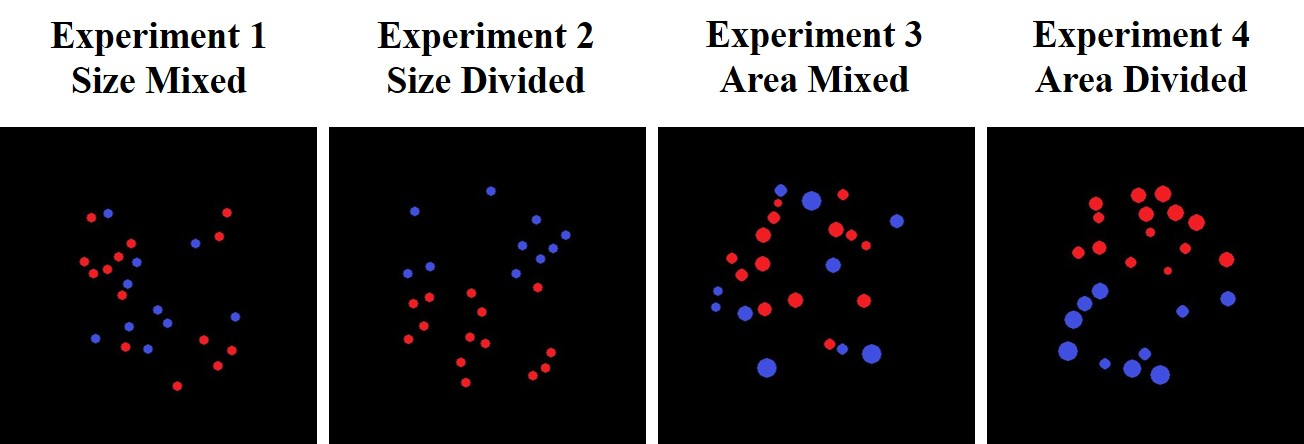
\includegraphics[scale = .45]{Figures/EstSystems/FIG4JPG.jpg}
\caption{Example stimuli from the fixed-item size, mixed color-set design of Experiment 1; the fixed item-size, divided color-set design of Experiment 2; the area-matched mixed color-set design of Experiment 3; and the area-matched divided color-set design of Experiment 4. Each example illustrates a double-target response-condition, where both the red and blue color-sets contain less than 20 items.}
\label{fig:ExpStim}
\end{figure}

\subsection{Participants}
Participants were undergraduate psychology students from the University of Newcastle, Australia, who completed a 90 minute experiment for three course-credits. The number and average age of participants in each of the four experiments are summarized in Table \ref{tab:Ch3_Participants}. All participants reported having normal or corrected to normal vision, and intact color vision.

\begin{table}[htb]
\centering
\caption{Summary table of participant number and mean age across experiments 1--4.}
\label{tab:Ch3_Participants}
\resizebox{\textwidth}{!}{%
\begin{tabular}{lll}
\hline
Experiment                       & Participants (Female) & Age (SD) years \\ \hline
1. Mixed Sets, Fixed Disc Size   & 21 (17)               & 22.67 (4.8)    \\
2. Divided Sets, Fixed Disc Size & 22 (20)               & 22.18 (5.37)   \\
3. Mixed Sets, Fixed Set Area    & 22 (14)               & 23.32 (3.67)   \\
4. Divided Sets, Fixed Set Area  & 21 (16)               & 22.19 (4.37)   \\ \hline \hline
\end{tabular}%
}
\end{table}

\subsection{Stimuli and apparatus}
The apparatus for each experiment was identical, with experiments only varying in stimuli. For simplicity, we will cover the stimuli and apparatus of Experiment 1 in detail, and then only detail the stimuli for each of the remaining experiments.

\subsubsection{Experiment 1}
Testing was conducted in the Newcastle Cognition Laboratory. Stimuli were presented on a 21.5inch Dell S2240L (60Hz) monitor. Stimuli were generated on a Dell Optiplex 7040 computer using python 2.7.14 and the Pygame 1.9.2b package. Responses were made using a standard `qwerty' keyboard. 

Stimuli comprised two sets of non-overlapping red and blue discs. Discs could appear within a central circular field of view, and the position of each disc within this area was sampled randomly (but without spatial overlap). At a viewing distance of 60cm, each disc subtended a visual angle of 0.14 degrees (0.15cm). The circular field of view subtended a visual angle of 9.52 degrees (10cm). Stimuli were presented on a black background. Red and blue colors had RGB values of (241, 29 ,34) and (64, 79, 223) respectively, and were matched for value and chroma using the Munsell color scheme \cite{Cochrane2014}, varying only by hue. Contrast and brightness effects were further controlled using a GLoptic spectis 1.0 photometer.

The first factorial manipulation was the presence or absence of an item-set less-than 20. The 2 (red set: target-present, absent) x 2 (blue set: present, absent) design results in four combinations of target and distractor presentations: double-target, double-distractor, red-target with blue-distractor, and blue-target with red-distractor. The simultaneous presentation of a target and distractor item-set will henceforth be referred to as the conflict-target condition. In addition to these four combinations, we also presented single-target and single-distractor item-sets, (e.g., red-target only, blue-target only, red-distractor only and blue-distractor only). This resulted in eight combinations of item-set presentations, as illustrated in Figure \ref{fig:DFP}. 

The number of red or blue discs presented in each color set varied by condition: target or distractor, high or low salience. The various combinations of response-type and salience-level are illustrated in Figure~\ref{fig:DFP}, with the color-printed integers 10, 14, 29 and 41 representing the set-size for the corresponding color (red or blue). For any one display, the minimum number of discs was 10 and the maximum number of discs (41 + 41) was 82.


\begin{figure}[htb]
\centering 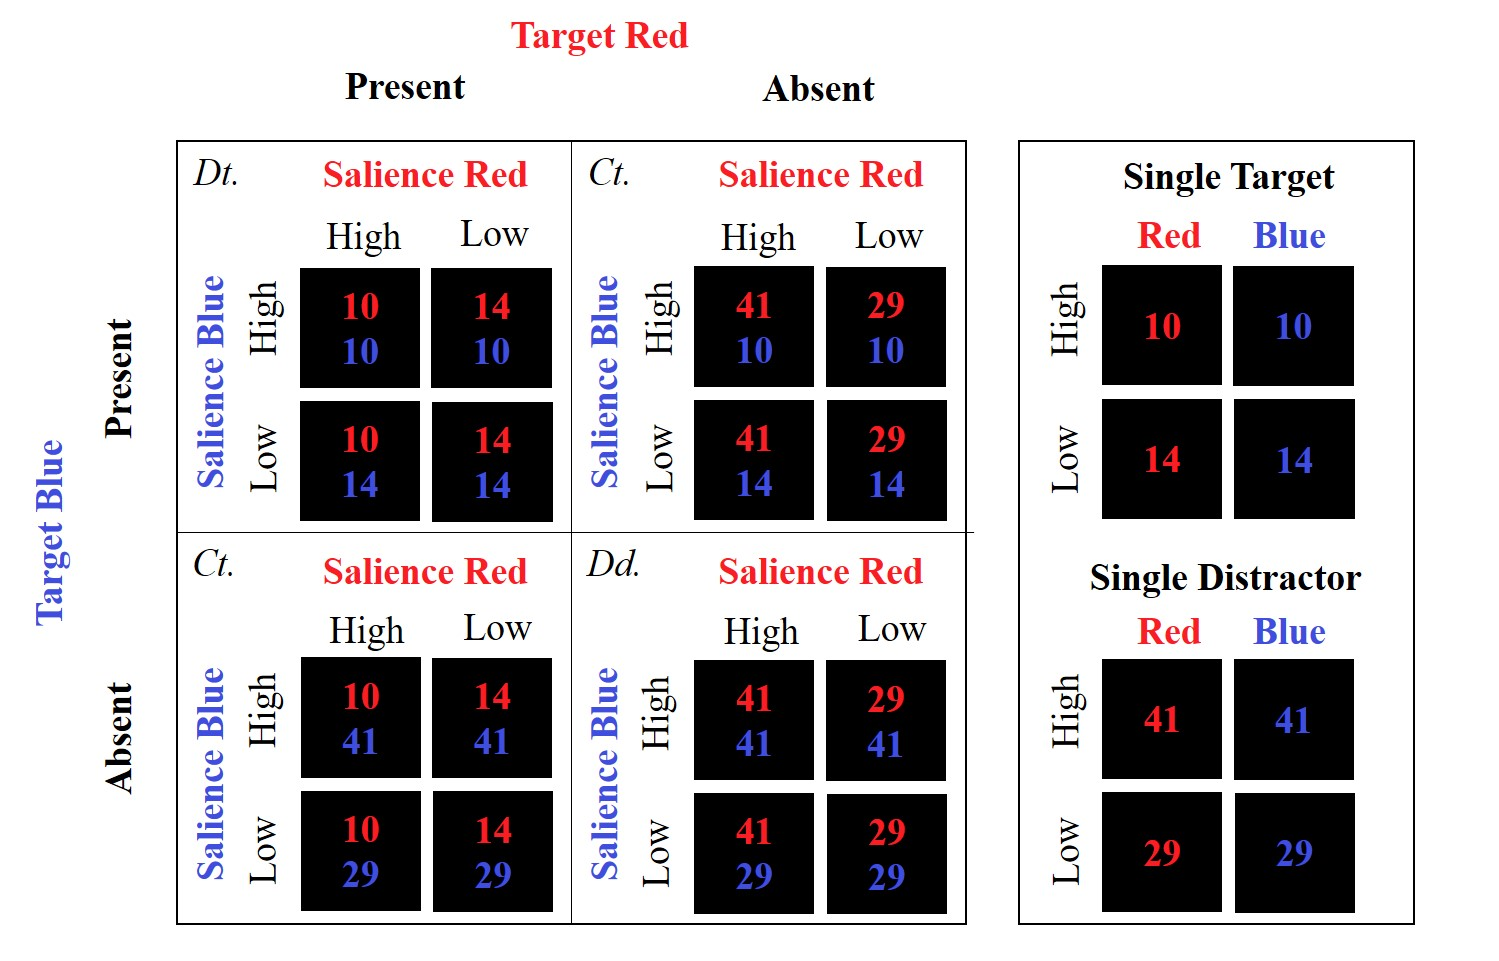
\includegraphics[width = \linewidth]{Figures/EstSystems/FIG5JPG.jpg}
\caption{Expanded double factorial paradigm. Factor one was the presence or absence of a target. Targets were item-sets less than 20. Distractors were item-sets greater than 20. This produced double-target ($Dt$), double-distractor ($Dd$), conflict-target ($Ct$), single-target and single-distractor item-sets. Factor two was the salience manipulation. High-salience item-sets (10 and 41) were further from the criteria (20) than low-salience item-sets (14 and 29). Each black square depicts a stimulus display. In displays where two item-sets were present (left outer-box), four salience combinations were possible: high-high, high-low, low-high and low-low. Single-stimulus displays (right outer-box) were either of high or low salience. Each integer (10, 14, 29 and 41) represent a single item-set presented in their associated color, see figure \ref{fig:ExpStim} for stimulus illustrations.}
\label{fig:DFP}
\end{figure}

\subsubsection{Experiment 2}
Experiment 2 aimed to assess whether the spatial grouping of each color-set aided in the capacity of the estimation-system, or altered the predominant processing-architecture. Stimuli were identical to those of Experiment~1, however each color set was confined to the top or bottom hemisphere of the central circular field-of-view (see second panel of Figure \ref{fig:ExpStim}). The top or bottom position of each color set was randomly selected on each trial. 

\subsubsection{Experiment 3}
Experiment 3 aimed to assess whether low-level covariates of quantity, specifically area, had an impact on the capacity or predominant processing architecture of the estimation system. Similar to Experiment 1, colored item-sets were intermixed within the circular stimulus display. Unlike Experiments 1 and 2, the size (radius) of each item varied. On each trial, the \textit{total} areas of the blue and red color-sets were matched. Color-set area was randomly sampled at the start of each trial and varied within a range of 1540--4620 pixels. This variation in total area was included to reduce the effect of item-size as a predictor of total item-set number. For example, if the total area was always equal to 3000 pixels, on average, the 10 item-set would have relatively large discs and the 41 item-set would always have small discs. Previously, \citeA{HALBERDA_2006} assessed the estimation system in a fixed-size experiment, a fixed item-set area experiment, and a fixed item-set circumference experiment, finding little difference between experimental accuracy or response-times. As such, we did not predict these low-level covariates to change the capacity or processing architecture results.


\subsubsection{Experiment 4}
Experiment 4 was an amalgamation of Experiments 2 and 3. It aimed to assess whether the spatial location of the color-sets and the low-level covariate of area, altered the capacity or predominant processing-architecture of the estimation-system. Experiment 4 controlled for the area of each color-set within a trial, in the same manner as Experiment 3. Similar to Experiment 2, stimuli were presented in either top or bottom hemispheres of the central circular field-of-view (see Figure \ref{fig:ExpStim}).

\subsection{Procedure}
Each participant completed a single 90 minute experimental session. Participants were presented with an information sheet and consent form and answered demographic questions regarding age, gender, handedness, vision and color-blindness. Participants were asked to complete a redundant-target estimation task, in which any display containing a target set (number of discs in set $<$ 20) called for a `yes', target-present response. Any display containing only distractor item-sets, (e.g., double-distractor or a single-distractor only item-set), called for a `no', target-absent response. Participants responded `yes' to the presence of a target with the `z' key and `no' to the absence of a target with the `/' key. Response keys were counter-balanced across participants.

At the start of each trial, participants were directed to look at a central fixation cross, presented for 500ms and followed by a 500ms blank screen. The stimulus display was then presented for 1000ms, followed by a mask for 500ms and a post-mask blank for 2500ms. From the onset of the stimulus, participants had 4000ms to make a response. The trial ended when the participant made a response or the trial timed-out at the conclusion of the response window. 

Participants completed one practice block and 15 experimental blocks, each containing 96 randomly ordered trials. Trial-by-trial accuracy feedback was provided during the practice block. Each block contained 12 double-target trials, 12 double-distractor trials, 24 conflict-target trials, 24 single-target trials and 24 single-distractor trials, presented in a random order. These trials were evenly distributed among the constituent salience levels. For example, three trials were presented from each double-target salience combination --- 12 in total. By comparison, six trials were presented from each of the red and the blue, single-target high and single-target low salience conditions --- 24 in total. Not including practice trials, each subject completed 180 double-target trials, 180 double-distractor trials, 360 conflict-target trials (180 target-red, 180 target-blue), 360 single-target trials (180 target-red, 180 target-blue) and 360 single-distractor trials (180 distractor-red, 180 distractor-blue). In total, subjects completed 1440 experimental trials with a 5:3 yes/no response bias. The probability of a target item-set in one color, (e.g., red), given a target item-set in the other color, (e.g., blue), was 0.33 \cite{mordkoff1991}.

\section{Data analysis}
Incorrect trials, and trials with response times less than 150 ms or greater than the 97.5$^{th}$ percentile were excluded from analysis. Participants' data were included if their total accuracy was $>80\%$ correct, \emph{and} their conditional accuracy in each of the six target conditions was $>66\%$. All repeated-measures ANOVAs were corrected for violations of sphericity, where appropriate, using the Greenhouse-Geisser correction. Post-hoc paired $t$-tests were corrected for family wise error using the Bonferroni method. 

Workload capacity was assessed through the redundant target effect \cite<RTE; >{miller1982divided, eidels2008similarity}, the capacity coefficient and resilience difference function. The RTE assesses the cost or gain associated with processing an additional, redundant target item-set, when compared to the processing of a single target item-set in isolation. A negative RTE indicates a cost to workload capacity. The RTE can be expressed as RTE = $min$(\mRT{RedTarget}, \mRT{BlueTarget}) - \mRT{DoubleTarget}, such that a negative RTE indicates a redundancy cost. The RTE was tested for significance at the cumulative distribution level through a series of non-parametric Kolmogrov-Smirnov (KS) tests, investigating the distribution ordering to determine whether $min$[$F_{RedTarget}$($t$), $F_{BlueTarget}$($t$)] $>$ $F_{DoubleTarget}$($t$). As the KS test is a conservative measure, we followed the method reported by \citeauthor{johnson2010systems} \citeyear{johnson2010systems} and adopted a more liberal alpha ($p$ $<$ 0.15) to determine significance.

Processing architecture was assessed for double-target conditions (where red and blue item-sets both satisfied the criterion and each contained less than 20 items) using the mean interaction contrast (MIC) and its distributional counterpart, the survivor interaction contrast [SIC($t$)]. The MIC distinguishes between parallel self-terminating (MIC $>$ 0), parallel exhaustive (MIC $<$ 0), and serial models (MIC = 0). Due to the construction of the MIC, a significance test of the interaction term between high and low salience levels can establish whether the model is parallel. The SIC($t$) can distinguish between the two parallel models, and additionally the serial self-terminating and serial exhaustive models, however requires selective influence to hold for each manipulation of salience at the level of the cumulative distribution. We tested a criterion for the presence of selective influence within double-target conditions for each subject individually using the following non-parametric KS tests \cite<alpha $p$ $<$ 0.15; see>{johnson2010systems}:

\noindent
\begin{align*}
S_{\rm LL}(t) &< \left\{S_{\rm LH},S_{\rm HL}\right\} \textrm{ is significant}\\
S_{\rm LL}(t) &> \left\{S_{\rm LH},S_{\rm HL}\right\} \textrm{ is not significant}\\
S_{\rm HH}(t) &> \left\{S_{\rm LH},S_{\rm HL}\right\} \textrm{ is significant}\\
S_{\rm HH}(t) &< \left\{S_{\rm LH},S_{\rm HL}\right\} \textrm{ is not significant}\\
S_{\rm HH}(t) &< S_{\rm LL}(\t)  \textrm{ is significant}
\end{align*}

Until fairly recently, inference on the SIC($t$) was limited to visual inspection. \citeauthor{houpt2010statSIC} \citeyear{houpt2010statSIC} developed null-hypothesis significance tests (NHST) to more formally diagnose deviations from a zero SIC. However, these tests are limited by the standard pitfalls of NHST. In particular, the `null' signature actually corresponds to the serial OR model, making direct inference about that model difficult under the NHST framework. More recently, \citeA{houpt2017bayesSIC} developed a non-parametric Bayesian approach for categorizing SIC($t$). The approach is based on a Dirichlet process that samples thousands of SIC functions based on the empirical probabilities of each condition at certain quantiles, and categorizes each sample based on which model shape it best approximates (as illustrated back in Figure \ref{fig:SIC}).

The Bayesian framework has the advantage of quantifying the strength of evidence for each model (allowing comparison of model weights), and also allows direct inference about the serial models. We implemented this Bayesian approach to help categorize our SIC models. We used a uniform prior on the model space such that the prior likelihood of sample corresponding to a given SIC state (neither, one, or both of a positive or negative deviation at some time \textit{t}) was equally likely. This uniform prior has the advantage of giving very weak evidence for all models in the case an SIC is truly uninformative, whereas the approach presented by \citeauthor{houpt2017bayesSIC} tended to show strong evidence of serial processing in such cases \cite{houpt2017bayesSIC}. To be sure, testing confirmed that using the uniform prior distribution did not hurt model recovery when applied to the simulated data from \citeauthor{houpt2017bayesSIC}'s (2017).

In addition to the SIC analyses, we implemented the hierarchical MIC estimation procedure introduced by \cite{houpt2017hierarchical}.
This analysis involved hierarchically estimating parameters of a gamma distribution for each subject's conditional response-time distribution, where the rate parameter of each distribution was constrained by a higher-order 'MIC state' model. This procedure allows a parametric evaluation of evidence for processing architecture at the MIC level --- serial (MIC = 0), parallel minimum-time (MIC $>$ 0) and parallel maximum-time (MIC $<$ 0). Using these two Bayesian approaches we were able to obtain converging Bayesian evidence for serial and parallel processing architectures using both non-parametric (Bayesian SIC), and parametric (Bayesian MIC) approaches. 

\section{Results}
In these results, we will focus on system capacity, conflict-target resilience (\ie architecture and workload), and target processing architecture. For clarity of exposition, experiments are presented together for each of the above sections.

\subsection{Group Means}
Participants with conditional accuracy $< 66\%$ or total accuracy $< 80\%$ were excluded from analysis. Three participants were excluded from Experiment 1 and Experiment 3, and two participants were excluded from Experiment 2 and Experiment 4 due to low accuracy. Accuracy was high for all remaining subjects in Experiment 1 (\Acc{0.94}{0.04}), Experiment 2 (\Acc{0.94}{0.03}), Experiment 3 (\Acc{0.93}{0.03}) and Experiment 4 (\Acc{0.93}{0.04}). Error rates were too low to afford statistically meaningful comparisons between response conditions. As such, the remaining results focus exclusively on our primary metric, response-time.

The following response-time results section focuses on red single-target (Rt), blue single-target (Bt) and double-target (Dt) responses, as these conditions form the basis of the subsequent workload capacity analysis. These response-sets are formed from the combination of their nested salience levels. Red single-target responses are formed from the high (H) and low (L) red target-salience levels, and double-target responses include combinations of HH, HL, LH and LL red-and-blue target-salience levels.

\subsubsection{Experiment 1: Fixed Sized Items, Mixed Color-Sets}
Mean response-time (mRT) results for Experiment 1 are plotted as black markers towards the left of Figure \ref{fig:MeanRTAcc}. Within the target conditions, there was a significant effect of workload (number of targets) on response-time (\Fval{1.47}{25}{27.34}{$<$ .001}, \etap{0.62}). Post-hoc paired sample $t$-tests showed red-target responses (\rt{551}{56}) were faster than double-target responses (\rt{589}{68}); \tval{17}{5.122}{$<$ .001}, $d$ = 1.21). Likewise, blue-target responses (\rt{546}{53}) were faster than double-target responses (\tval{17}{6.063}{$<$ .001}, $d$ = 1.43). Red-target and blue-target responses did not significantly differ (\tval{17}{1.325}{= 0.20}, $d$ = 0.31). Bonferroni corrections were used for multiple comparisons, where appropriate. 

\begin{figure}[htb]
\centering 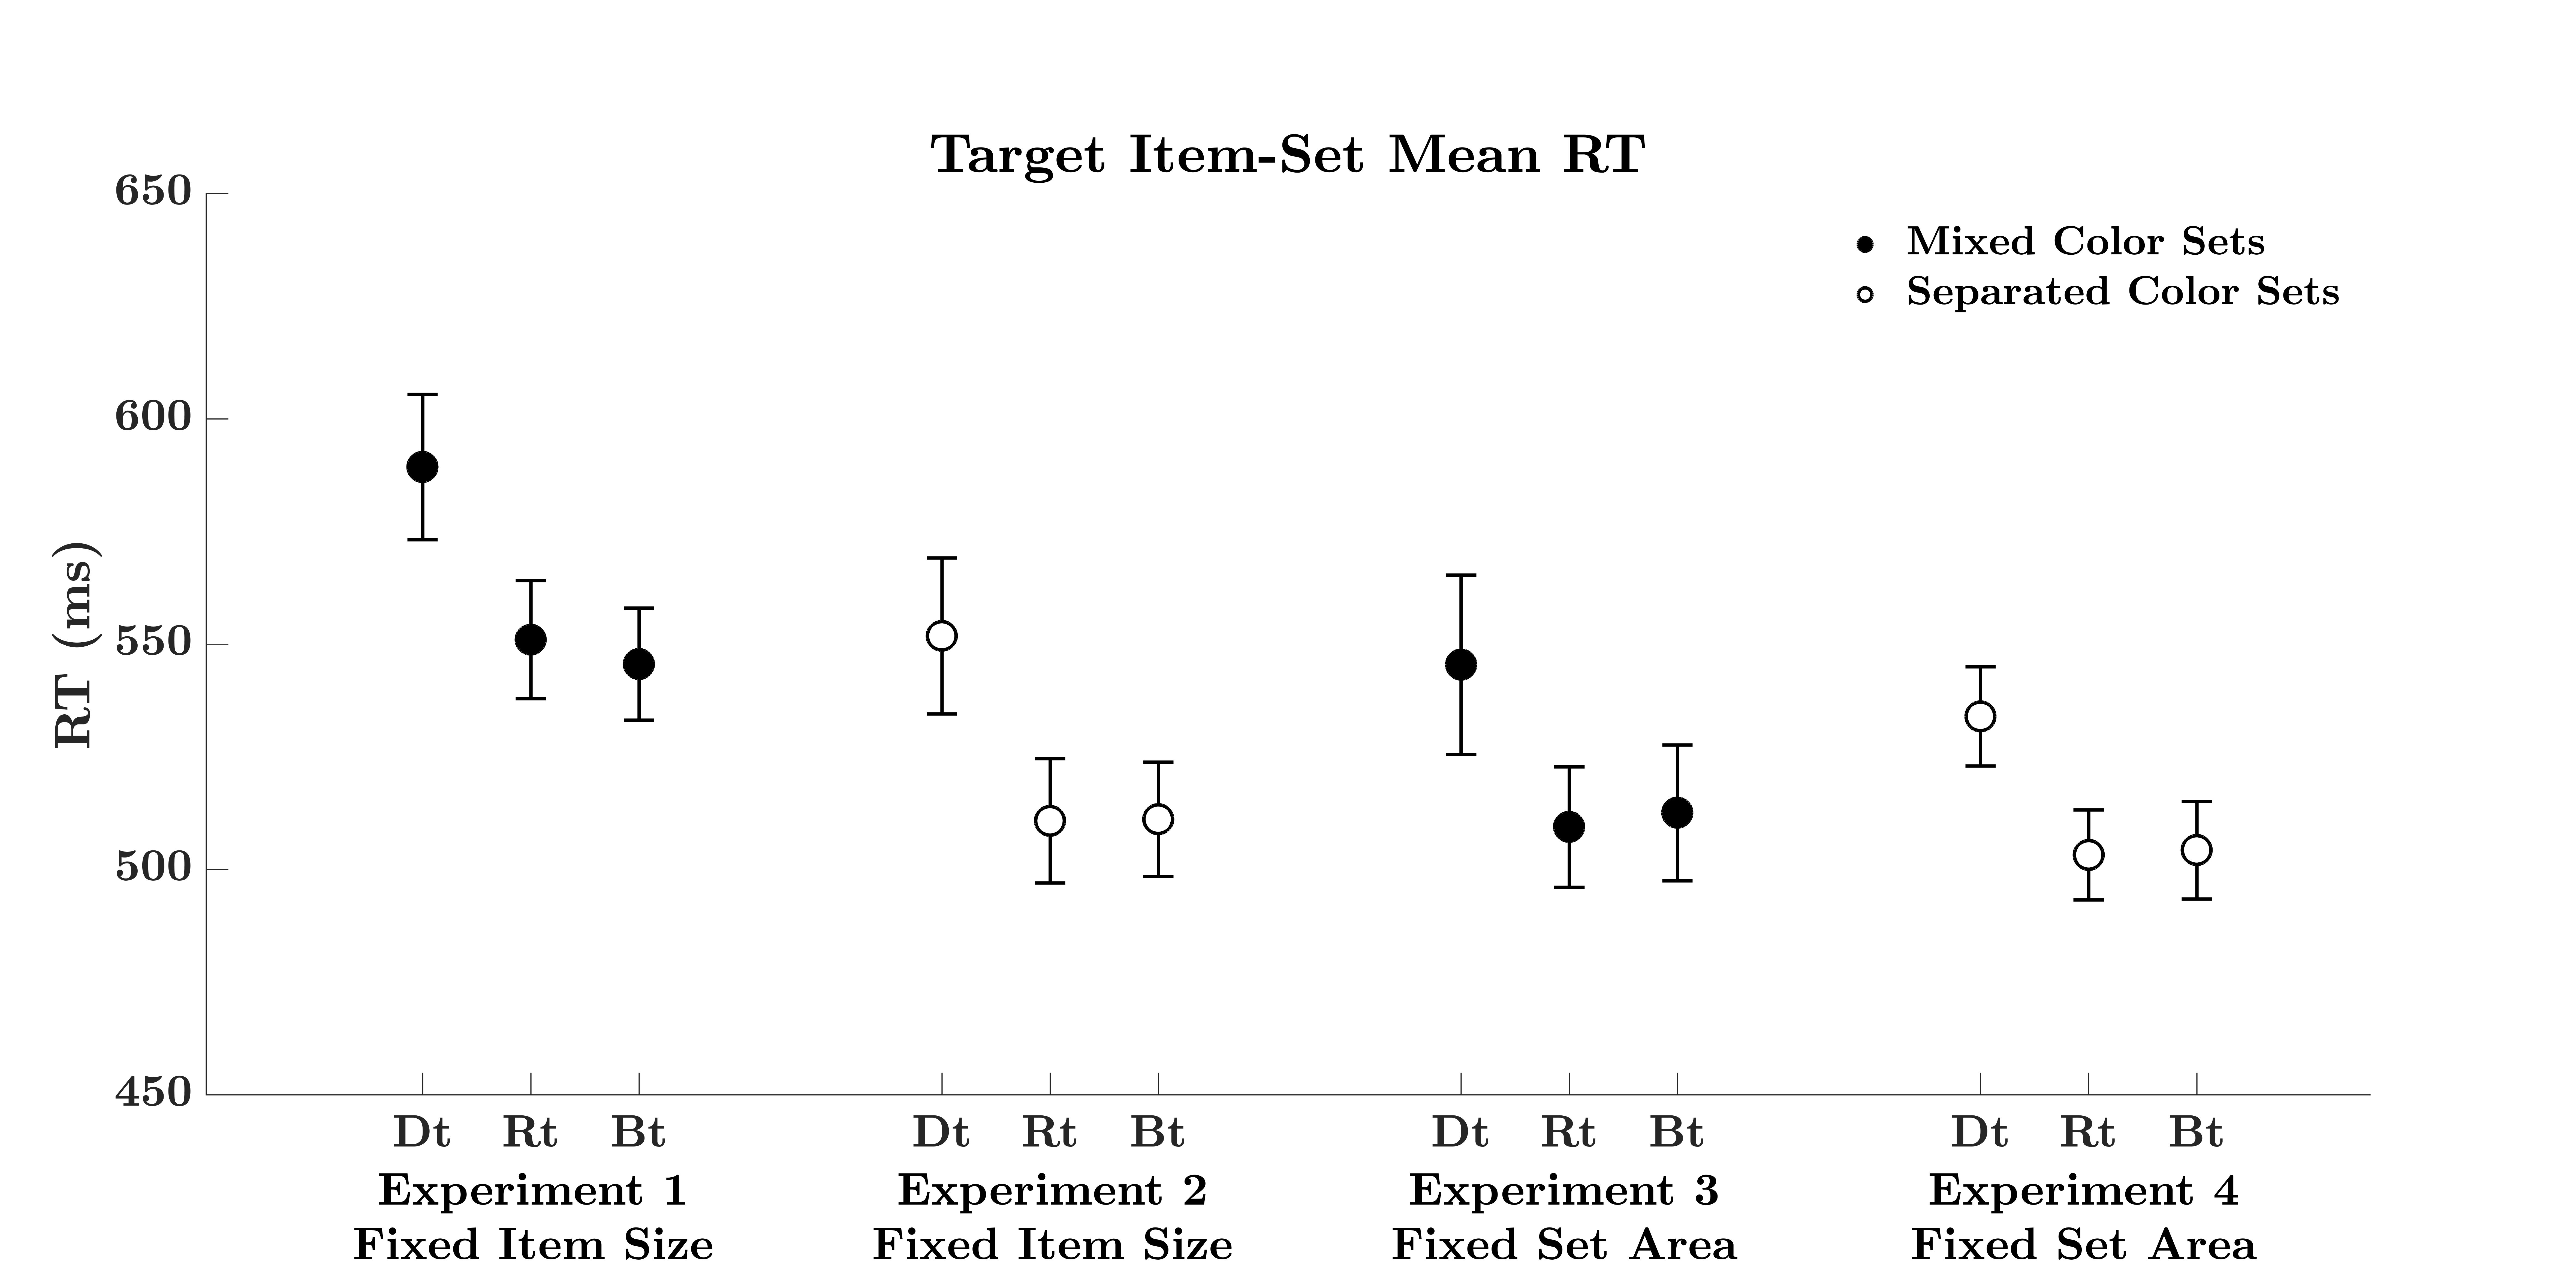
\includegraphics[width=\linewidth]{Figures/EstSystems/FIG6JPG.jpeg}
\caption{Mean response-time plots for double-target (Dt), red single-target (Rt) and blue single-target (Bt) response sets, across Experiments 1 ($N$ = 18), 2 ($N$ = 20), 3 ($N$ = 19) and 4 ($N$ = 19). Plots illustrate the slowing of double-target responses within each experiment, relative to their single-target counterparts. Error bars represent $\pm$ one standard error of the mean.}
\label{fig:MeanRTAcc}
\end{figure}

\subsubsection{Experiment 2: Size Divided Color-Sets}
Mean response times for Experiment 2 are plotted as white markers towards the left of Figure \ref{fig:MeanRTAcc}. There was a significant effect of target-type on RT (\Fval{1.22}{23.25}{36.08}{$<$ .001}, \etap{0.66}). Red-target responses (\rt{511}{62}) were faster than double-target responses (\rt{551}{77}; \tval{19}{6.84}{$<$ .001}, $d$ = 1.53), and blue-target responses (\rt{511}{57}) were faster than double-target responses (\tval{19}{5.807}{$<$ .001}, $d$ = 1.3). Red and blue single-target responses were not significantly different (\tval{19}{-0.136}{= 0.89}, $d$ = -0.03).

\subsubsection{Experiment 3: Area Mixed Color-Sets}
Mean response times for Experiment 3 are plotted as black markers towards the right of Figure \ref{fig:MeanRTAcc}. There was a significant effect of target-type on response-time (\Fval{1.44}{25.89}{12.82}{$<$ .001}, \etap{0.42}). Post-hoc paired $t$-tests revealed red-target responses (\rt{509}{58}) were faster than double-target responses (\rt{545}{87}); \tval{18}{4.184}{$<$ .01}, $d$ = 0.96), and blue-target responses (\rt{513}{66}) were faster than double-target responses (\tval{18}{3.504}{$<$ .01}, $d$ = 0.8). Red-target and blue-target responses were not significantly different (\tval{18}{-0.638}{= 0.53}, $d$ = -0.15).

\subsubsection{Experiment 4: Area Divided Color-Sets}
Mean response times for Experiment 4 are plotted as white markers towards the right of Figure \ref{fig:MeanRTAcc}. In line with previous experiments, there was a significant effect of target-type on response-time (\Fval{1.46}{26.28}{30.39}{$<$ .001}, \etap{0.63}). Post-hoc paired $t$-tests showed red-target responses (\rt{503m}{44}) were faster than double-target responses (\rt{534}{48}); \tval{18}{6.414}{$<$ .001}, $d$ = 1.47), and blue-target responses (\rt{504}{48}) were faster than double-target responses (\tval{18}{5.529}{$<$ .001}, $d$ = 1.27). Red-target and blue-target responses were not significantly different (\tval{18}{-0.362}{= 0.72}, $d$ = -0.08).

\subsection{Redundant Target Effects}
As reported in Group Means section, double-target responses were significantly slower than single-target responses. This $redundancy$ $cost$, displayed as a negative RTE, was observed in all experiments and suggests that the addition of a second target slows the estimation-system, a hallmark of limited capacity processing. However, a redundancy cost at the group level does not dictate a redundancy cost for each subject. The following section examines the direction and significance of the redundant target effect for each subject.

\subsubsection{Experiment 1: Size Mixed Color-Sets}
Individual redundant target effects and corresponding significance values are plotted in the top-left panel of Figure \ref{fig:GroupRTE}. Seventeen subjects in Experiment 1 recorded a significant redundancy cost at the distributional level (KS $<$ .15), suggesting these individuals experienced capacity limitations when processing two target item-sets. One subject exhibited a redundancy cost, however, did not reach significance at the level of the distribution.

\begin{figure}[hbt]
\centering 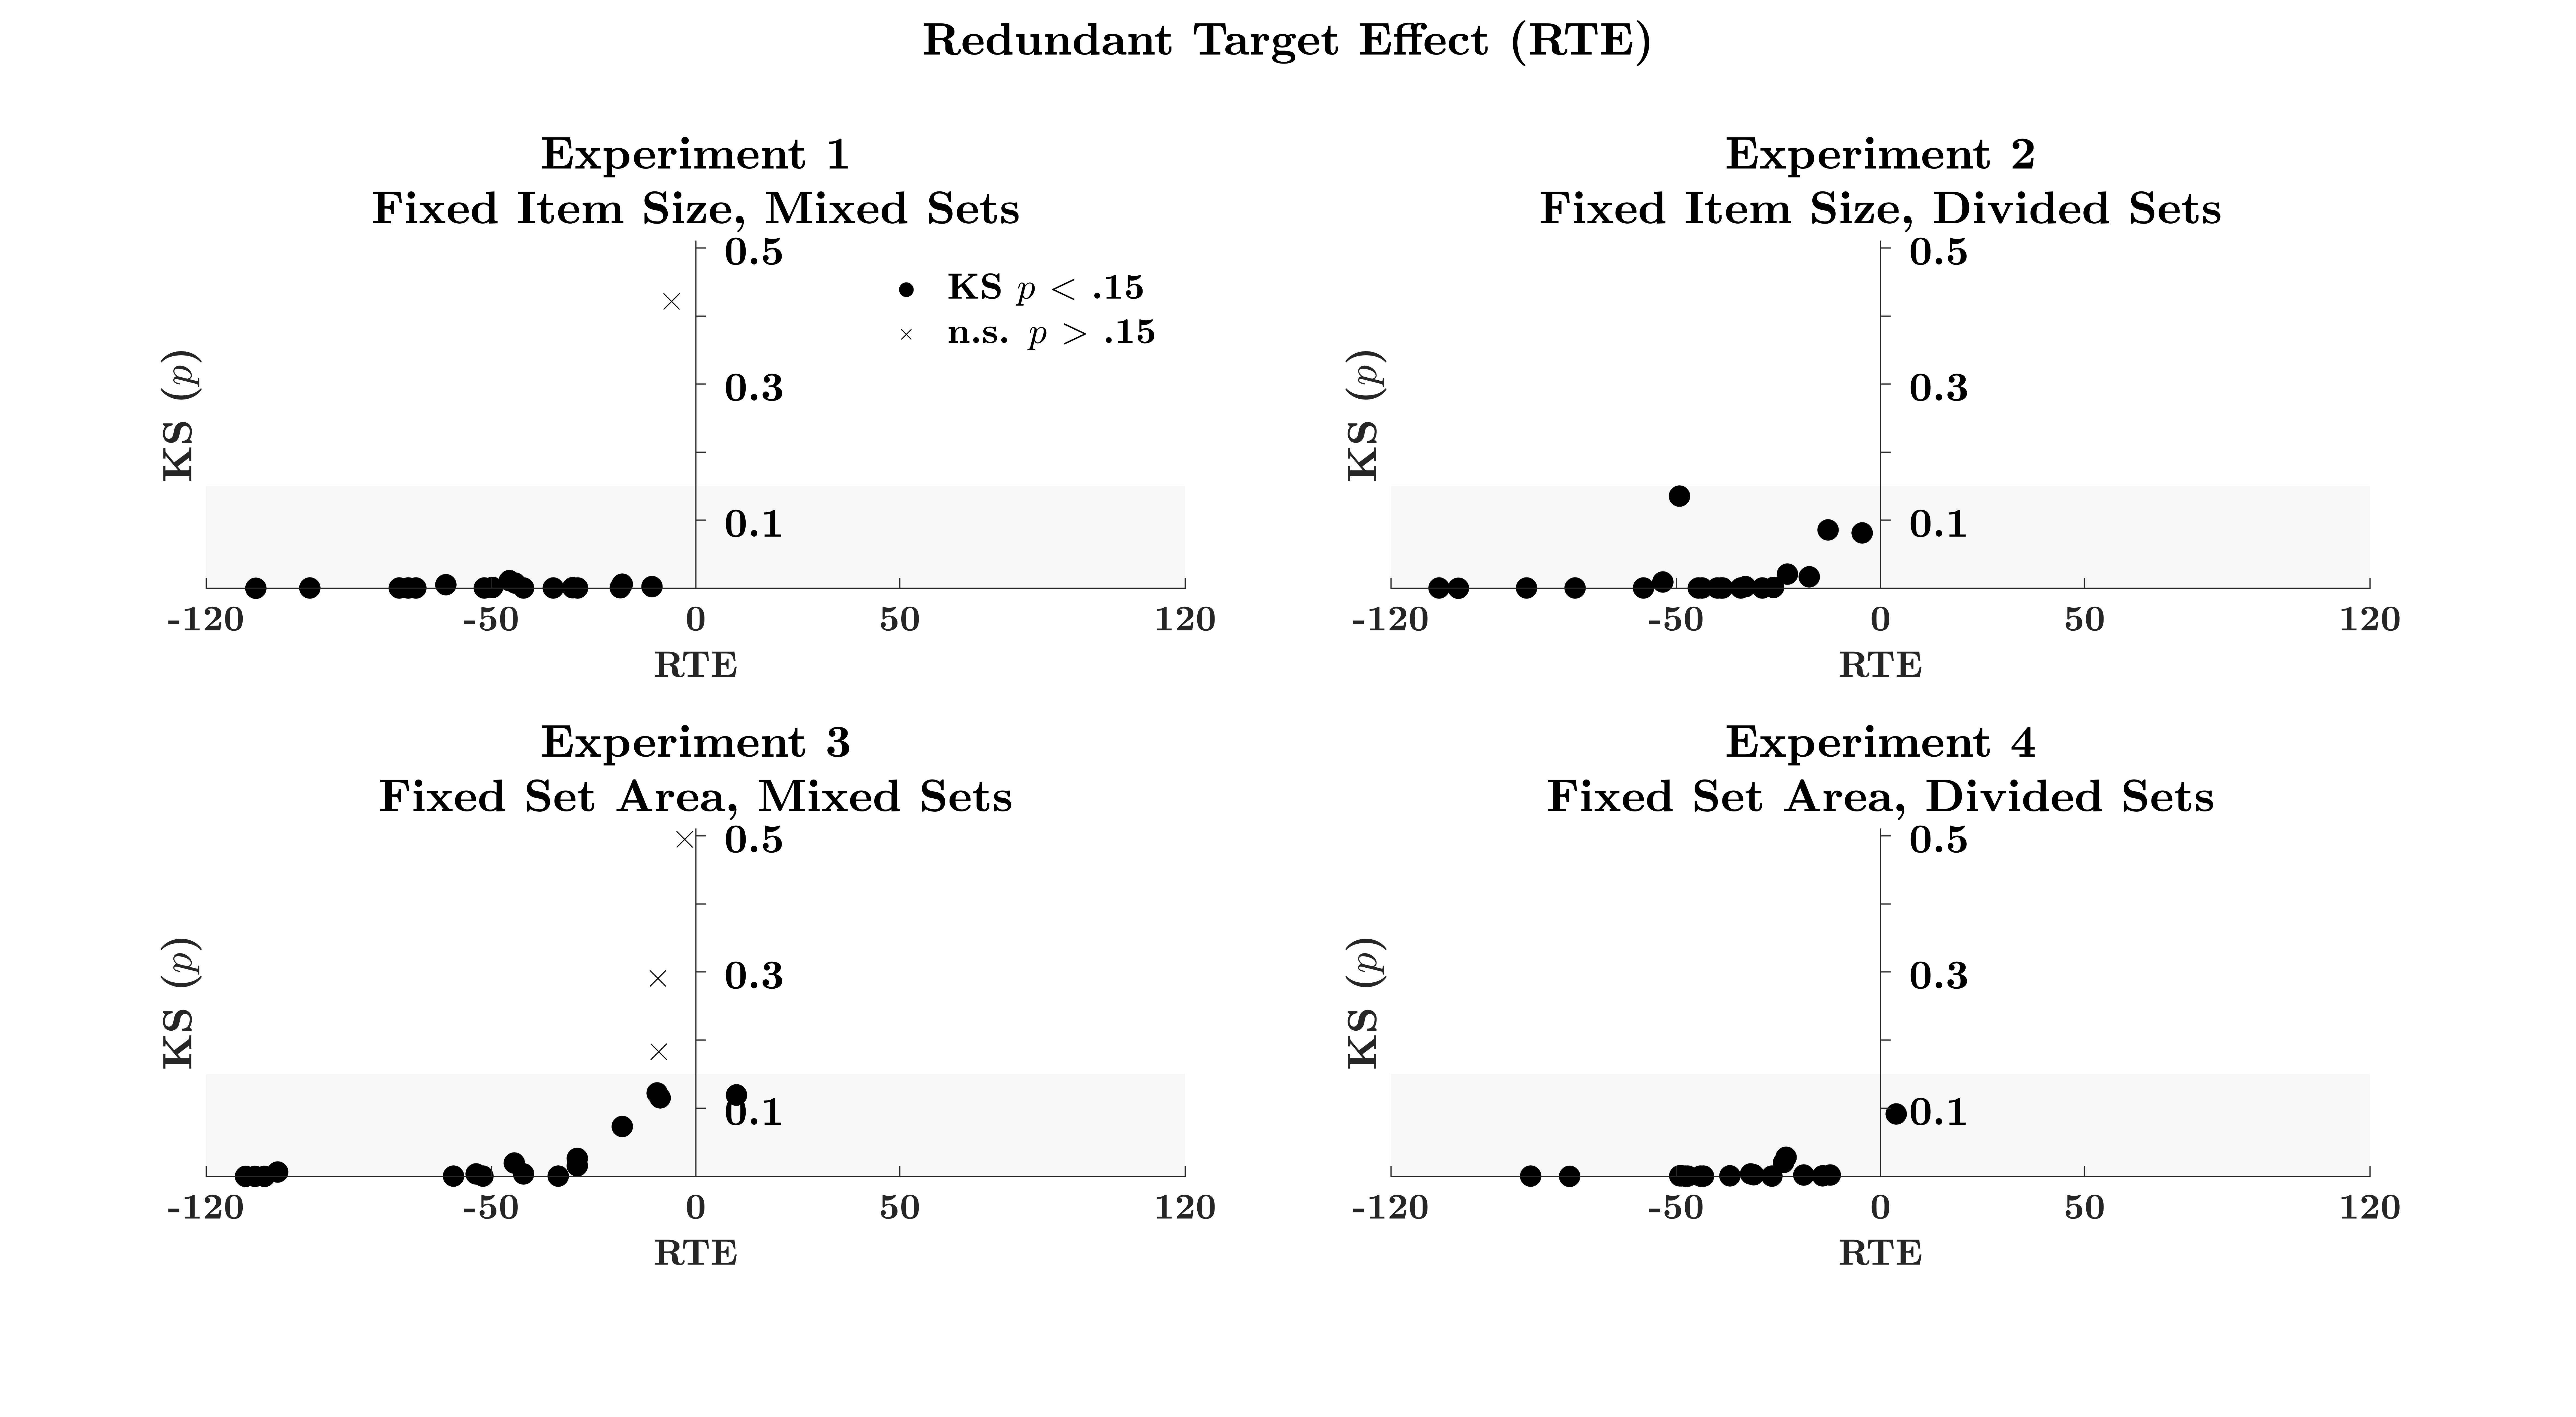
\includegraphics[width=\linewidth]{Figures/EstSystems/FIG7JPG.jpeg}
\caption{Significance values for individual subject's redundant target effects (RTE) plotted separately for Experiments 1 ($N$ = 18), 2 ($N$ = 20), 3 ($N$ = 19) and 4 ($N$ = 19). Negative RTE values denote a redundancy cost. Each subject is plotted as an individual marker, black markers indicate a significant RTE (KS $p < .15$), and X markers indicate a non-significant RTE (KS $p > .15$). Across the four experiments, most subjects exhibited a significant redundancy cost. \newline \emph{\bf Note:} One outlier was excluded from the Experiment 4 RTE plot, RTE = -10 and $p = 0.63.$}
\label{fig:GroupRTE}
\end{figure}


\subsubsection{Experiment 2: Size Divided Color-Sets}
Individual subject's redundant target effects and corresponding significance values are plotted in the top-right panel of Figure \ref{fig:GroupRTE}. All 20 subjects exhibited significant redundancy costs at the level of the distribution (KS $<$ 0.15). 

\subsubsection{Experiment 3: Area Mixed Color-Sets}
Individual subject's redundant target effects and corresponding significance values are plotted in the bottom-left panel of Figure \ref{fig:GroupRTE}. Fifteen subjects exhibited a significant redundancy cost at the level of the distribution. One participant recorded a redundancy $gain$ (positive RTE) at the level of the distribution, in contrast to the trend of most subjects in this experiment. Three subjects recorded a redundancy cost, but did not reach significance at the distribution level.

\subsubsection{Experiment 4: Area Divided Color-Sets}
Individual subject's redundant target effects and corresponding significance values are plotted in the bottom-right panel of Figure \ref{fig:GroupRTE}. Eighteen subjects recorded a significant redundancy cost at the level of the distribution. One subject recorded a redundancy cost but did not reach significance at the level of the distribution. This subjects was removed as an outlier from the Experiment 4 RTE plot and recorded an RTE = -10 ($p = 0.63$). 

\subsection{Capacity Coefficient}
Nearly all participants, in all four experiments, showed a significant redundancy cost (negative RTE) at the level of the distribution when estimating two target item-sets. The ubiquity of this finding suggests that the estimation of multiple item-sets is a limited capacity process, experienced by all individuals regardless of the perceptual covariate of item-set area, or whether item-sets were spatially overlapping or separate. For interpretation of individual subject's workload capacity across the entire response-time range, we may also consider the capacity coefficient. The capacity coefficient allows clear interpretation of performance limitations, as it assays performance against an established benchmark (unlimited capacity, independent-channels parallel model). 

Group mean and individual capacity coefficient (C($t$)) values for Experiments 1--4 are plotted in Figure \ref{fig:GroupCapacity}. Focusing on the group mean \Ct results from Experiment 1 (top-left panel), \Ct $<$ 1 for all of the response-time range, suggesting a limited workload capacity processing system. Furthermore, \Ct hovers below the Grice lower-bound for all of the response-time range. This suggests a system with severe capacity limitations. In line with the group results, all individual \Ct values (illustrated by gray markers) also hover at \Ct $<$ 1 and suggest limited workload capacity. Individual low-bounds present at approximately \Ct = 0.5, with all individual \Ct scores resting at or below the low-bound for the majority of the response-time range (individual \Ct plots for each experiment can be found in the supplementary materials, Figures \ref{fig:Indiv_Cap_Ex1}--\ref{fig:Indiv_Cap_Ex4}). In line with the group results, this suggests most individuals experienced severe capacity limitations when estimating multiple item-sets. Results from Experiments 2--4 show similar trends and support severely limited workload capacity processing systems in all subjects.

\begin{figure}[tbh]
\centering 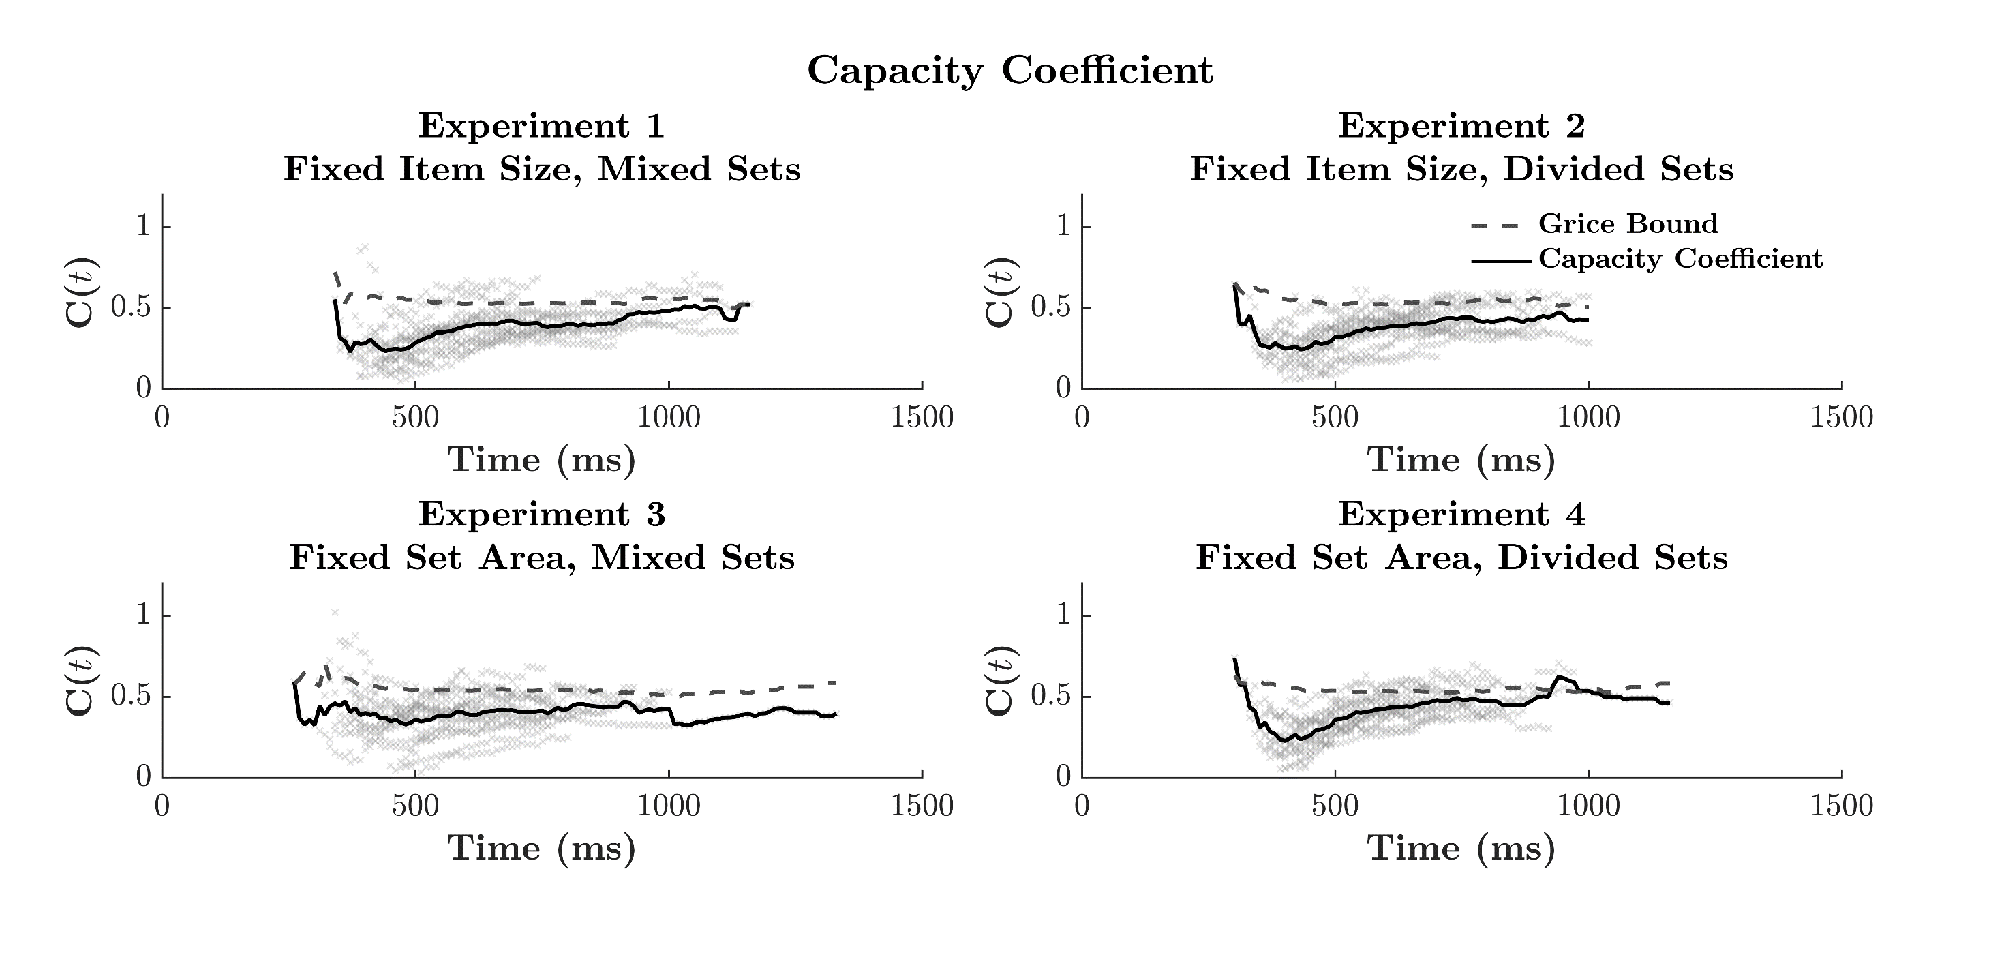
\includegraphics[width=\linewidth]{Figures/EstSystems/FIG8JPG.pdf}
\caption{Capacity coefficient (C($t$)) plots for target-present responses in Experiments 1--4. Group mean \Ct is plotted in black with the Grice lower-bound, an estimate of severe capacity limitations, depicted by the dashed line. Individual participant \Ct values are illustrated by gray markers and mostly fall at or below the group Grice bound, indicating severe capacity limitations across all experiments.}
\label{fig:GroupCapacity}
\end{figure}

Analysis of the capacity coefficient extends previous RTE analysis, showing that all subjects estimated multiple target-sets with limited workload capacity. Furthermore, performance of most subjects was at or below the Grice-bound, suggesting they may have experienced capacity limitations typically associated with serial processing architectures. We now consider the unique assessments of processing architecture and workload, provided by the resilience difference function, and compare these to our capacity coefficient results. 

\subsection{Resilience Function Analysis} 
Resilience difference (R$_{diff}$($t$)) values for the group mean as well as individual subjects, for low target-salience trials on each of the four experiments, are plotted in Figure \ref{fig:RdiffLow}. Interpretation of these results can be aided by comparison to \Rd predictions, presented in Figure \ref{fig:Rd}. Focusing on Experiment 1 group mean, \Rd hovers around zero, for most of the response-time range. This aligns with the prediction of a parallel minimum-time unlimited-capacity processing system. 
In line with the group results, most individual \Rd values (illustrated by gray markers) hover around \Rd = 0. Results from Experiments 2--4 show similar trends, in line with the predictions of a parallel minimum-time unlimited-capacity model. We replicated the \Rd analysis for high target-salience, and the results were again similar, in line with a parallel minimum-time unlimited-capacity processing system (see Figure \ref{fig:RdiffHigh} in the supplementary materials). Overall then, there seem to be some discrepancy between the capacity coefficient results, which support severely limited workload-capacity (potentially associated with serial architectures), and the resilience difference results, which support unlimited capacity that is often associated with parallel architectures. The fidelity of these claims can be directly assess through our next system measures, the MIC and SIC. 

\begin{figure}[tbh]
\centering 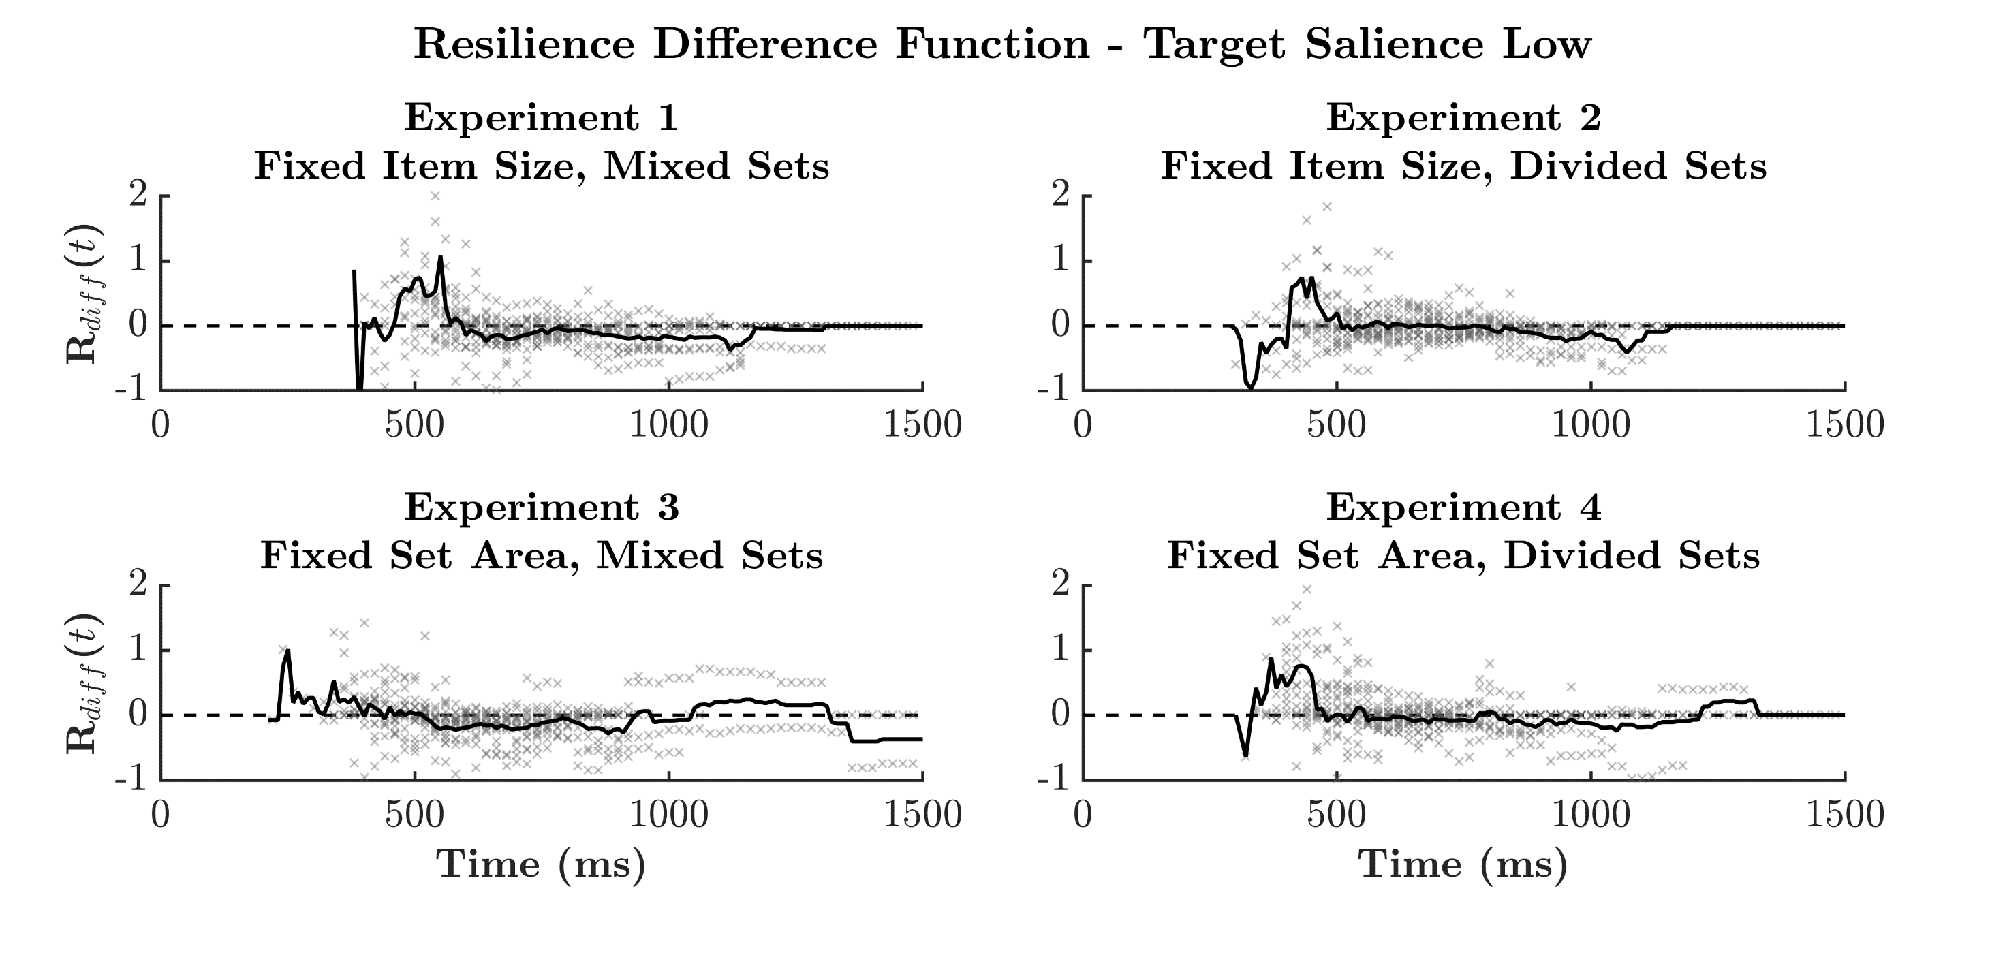
\includegraphics[width=\linewidth]{Figures/EstSystems/FIG9JPG.pdf}
\caption{Resilience difference plots for Experiments 1 – 4 when target salience is low. Black lines depict the average resilience difference function across subjects, while grey markers illustrate individual subject’s resilience difference functions. Average plots show a trend towards \Rd = 0, supporting predictions made by an unlimited-capacity parallel minimum-time processing system.}
\label{fig:RdiffLow}
\end{figure}

\subsection{Double-Target Processing Architecture}
In the following section, we report the MIC and SIC calculated from the response-time differences between salience manipulations --- high-high (HH), high-low (HL), low-high (LH) and low-low (LL) --- nested within the double-target response type. For valid interpretation, the mean interaction contrast (MIC) requires a successful manipulation of salience within both color-sets. This was assessed through a between-subject ANOVA conducted separately for each subject. For the MIC, a statistical interaction between the salience levels of each color-set acts as a test for parallel processing architectures and is therefore reported. Interpretation of the survivor interaction contrast (SIC) requires selective influence to hold at the level of the survivor functions (see the Data Analysis section for details). These tests were completed for each subject, and only subjects who met the criteria for selective influence are reported in Table \ref{table:Exp1_DT}. Finally, we report the Bayes factor for the winning MIC model, as MIC group posterior and the associated best MIC model fit. To foreshadow the outcomes, only a limited number of subjects satisfied the included criteria and could be categorized by processing architecture. For clarity of exposition, we first summarize the results of classified subjects across all experiments, then present a breakdown by individual subjects. 

MIC values for subjects who met SIC and MIC inclusion criteria in Experiments 1--4 are illustrated in the left panel of Figure \ref{fig:MICandProp_AB}. The majority of subjects in each experiment recorded a positive MIC value, supporting parallel minimum-time processing architectures. The right panel of Figure \ref{fig:MICandProp_AB} shows the proportion of each architecture, using the Bayesian SIC and hierarchical Bayesian MIC methods. Each bar represents the total number of (classified) subjects in a given experiment, and the shaded regions mark the relative proportion of subjects based on the way they enumerated two target sets (in parallel, serial). As expected, parallel processing architectures were applied by a majority of subjects in all experiments. Minimum-time stopping-rules were most common in Experiments 1--3, while in Experiment 4 most subjects used a maximum-time stopping rule. Individual results are  presented next. 

\begin{figure}[hbt]
\centering 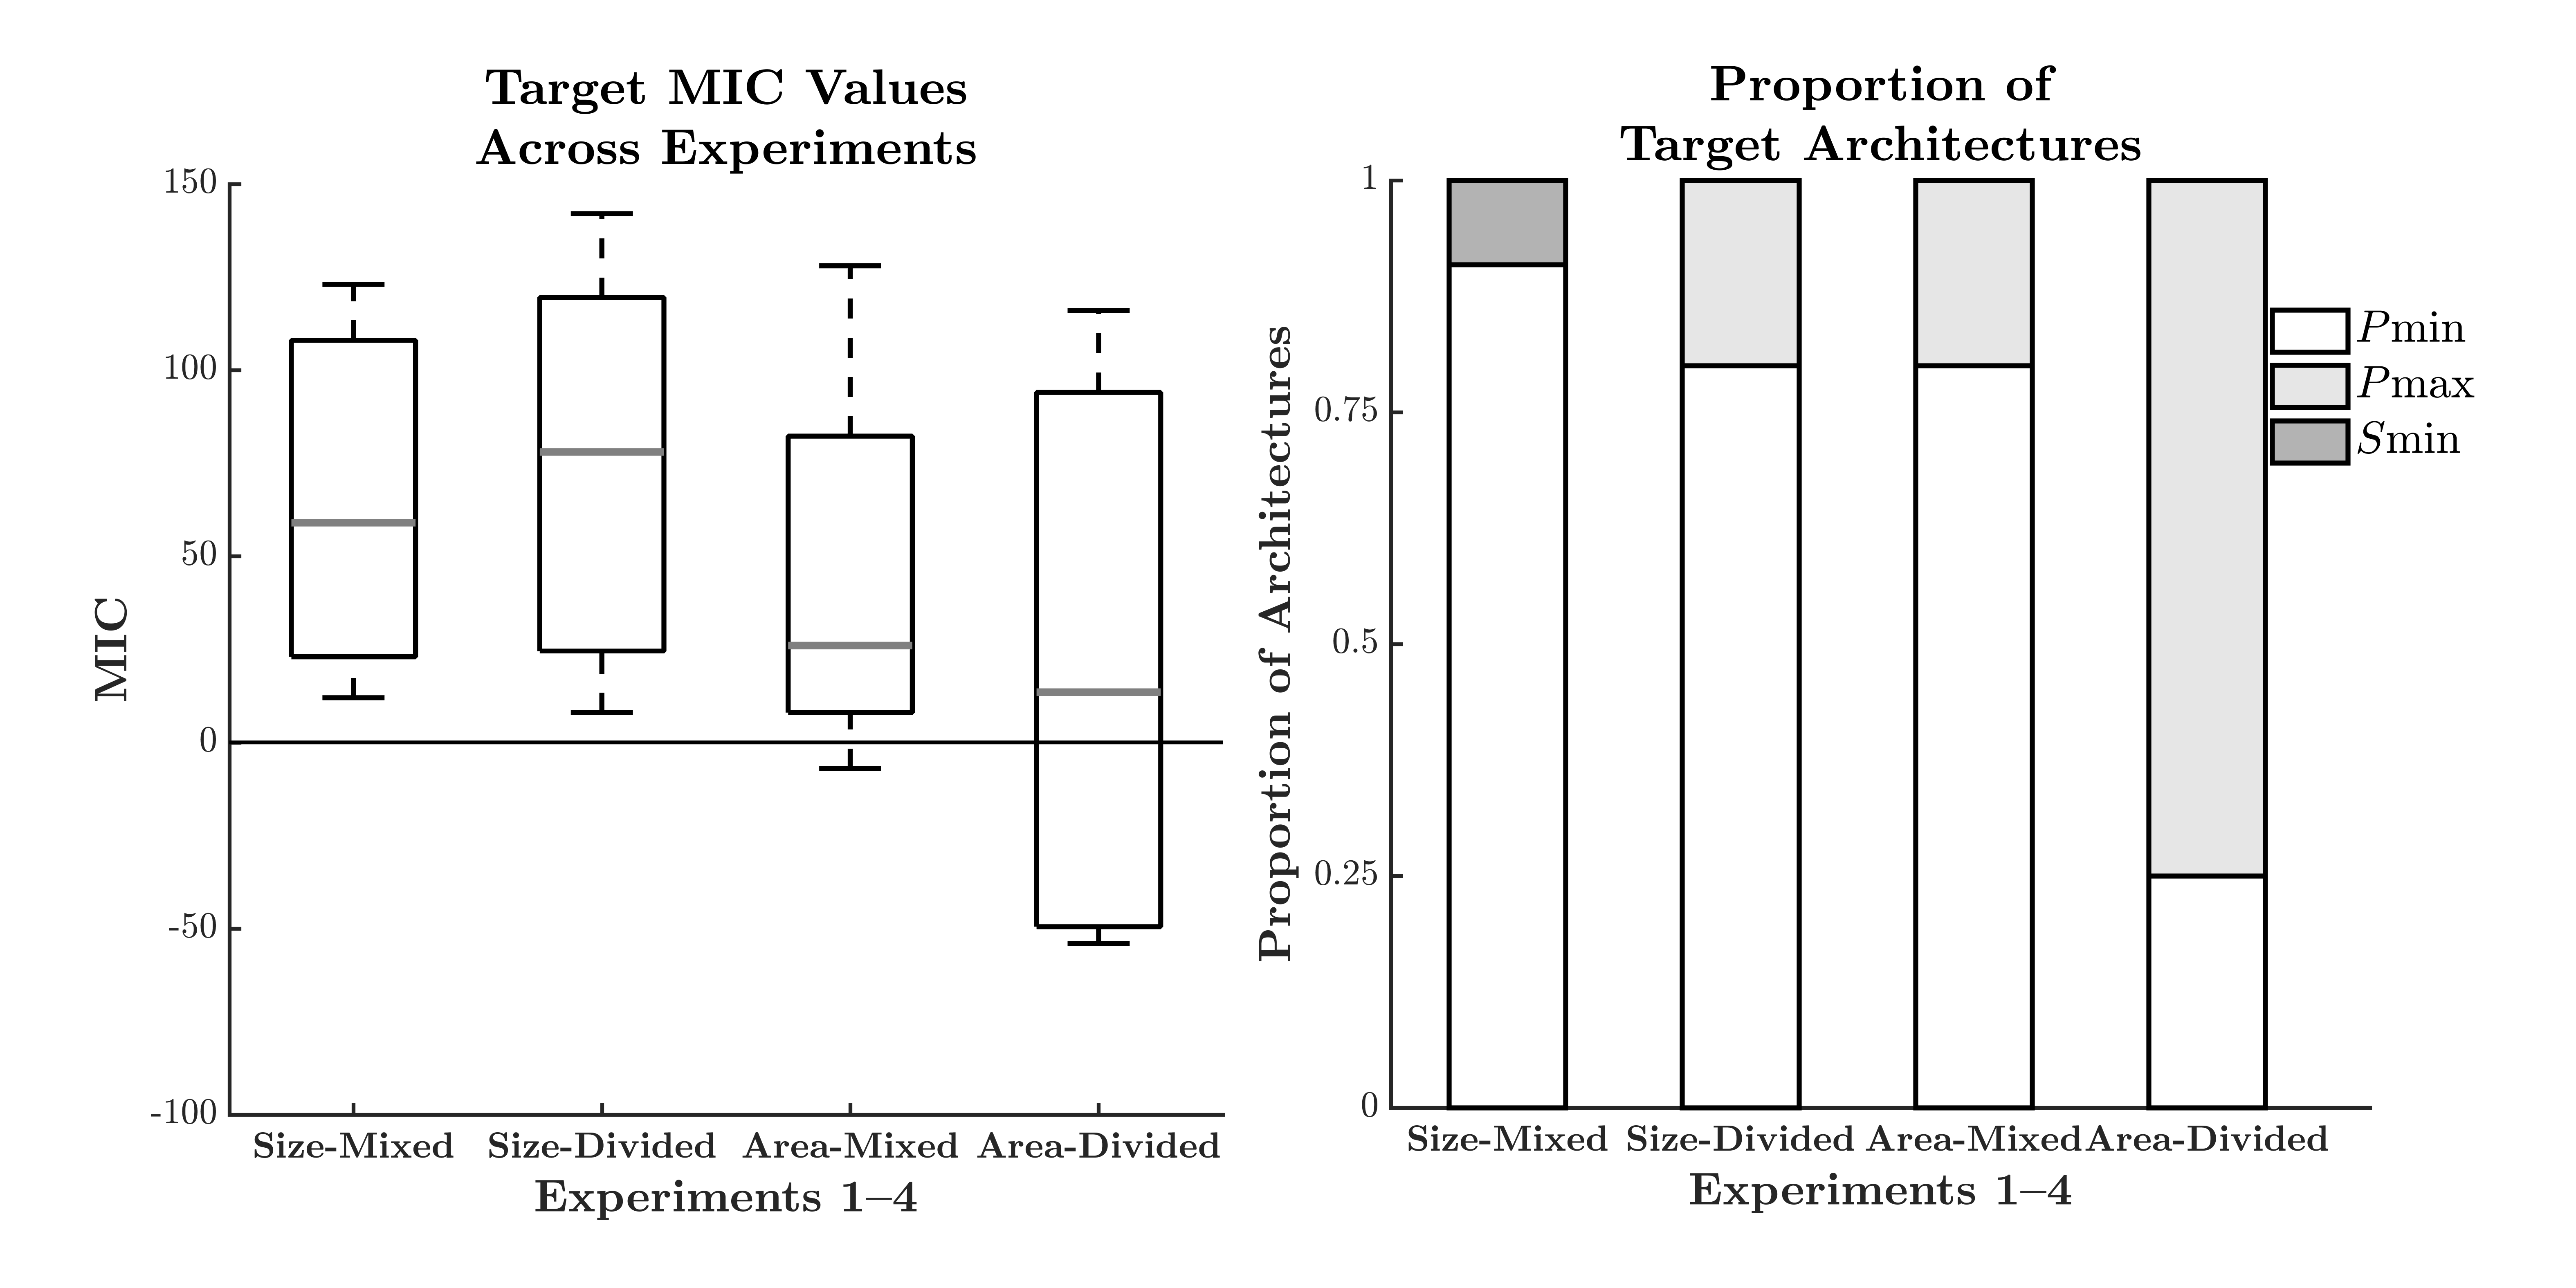
\includegraphics[width=\linewidth]{Figures/EstSystems/FIG10JPG.jpg}
\caption{MIC values (left) and the proportion of categorized processing architectures (right) for subjects in Experiments 1--4. Proportions are relative to the total number of subjects who could be classified using MIC and SIC significance testing. Ten subjects were categorized in Experiment 1, five subjects in Experiment 2, five subjects in Experiment 3 and four subjects in Experiment 4. \\ \textbf{Note.} $P$min = parallel minimum-time, $P$max = parallel maximum-time, $S$min = serial minimum-time.}
\label{fig:MICandProp_AB}
\end{figure}

\subsubsection{Experiment 1: Fixed Size, Mixed Color-Sets}
Individual MIC and SIC results are reported in Table 1, along with each subjects categorized candidate architecture. Subject categorization started with assessment of target salience effects. For each subject we tested for a main effect of red-target salience (R) and blue-target salience (B). Due to the construction of the MIC, a significant interaction of red-target and blue-target salience provides supportive evidence of a parallel processing architecture, while MIC valence indicates the stopping-rule. 


Stopping-rule refers to whether only one item-set (minimum-time rule) or both item-sets (maximum-time rule) need to be enumerated before a correct response may be given. This is different than the localized search-strategy employed when enumerating items \textit{within} each set. All reported subjects met the criteria for selective influence at the level of the distributions, assessed through a series of non-parametric KS test (see Data Analysis).

Subjects were categorized based on their SIC functions, classified using the newly developed non-parametric Bayesian SIC assessment techniques provided by \citeA{houpt2017bayesSIC}, supplemented by visual inspection of the MIC and ANOVA results\footnote{MIC interpretation was aided by consideration of MIC processing architecture plots. Visual assessment of the MIC plot has been beneficial in previous studies when categorizing processing architectures, however, is less robust than our recent method of classification, which utilizes the SIC.}. The new Bayesian SIC assessment techniques of \citeA{houpt2017bayesSIC} categorizes the subject SIC by processing architecture and stopping-rule, and further provides a model probability for observing a given processing architecture, (e.g., parallel minimum-time), relative to the four alternative architectures, (i.e., parallel maximum-time, coactive, serial minimum-time and serial maximum-time). As such, our criteria for a conclusive model architecture was determined via Bayesian SIC categorization where the candidate model displayed a selection probability greater than $0.5$, (i.e., where the candidate model was deemed more probable than all alternative model accounts). Finally, our results were augmented by a hierarchical Bayesian MIC analysis \cite{houpt2017hierarchical}, which takes into account data across all valid subjects in each experiment. For simplicity, we report the Bayes factor (BF$_{10}$) in favor of the best fitting model, identified in the far right columns of Table \ref{table:Exp1_DT}. 

\begin{table}[htb]
\caption{Individual double-target MIC and SIC results from Experiment 1. From left to right, ANOVA main effects for red target salience (R) and blue target salience (B), MIC value and interaction significance,  Bayesian SIC model probabilities and associated architectures, and Bayes factor values from the hierarchical MIC analysis with associated processing architectures. Note, P - Parallel, S - Serial.}
\centering 
\begin{tabular*}{\textwidth}{l @{\extracolsep{\fill}} lllllll}
\hhline{-------}
\textbf{Sub  } & \textbf{\begin{tabular}[c]{@{}c@{}}Main \\ Effects\end{tabular}} & \textbf{MIC} & \textbf{SIC} $\mathbb{P}$ & \textbf{SIC Model} & \textbf{BF$_{10}$} & \textbf{MIC Model} \\  
\hhline{-------}
101 & R \& B & 53*    & \textbf{0.73} & \textbf{P Min-Time} & \textbf{10.69}  & \textbf{P Min-Time} \\ 
102 & R \& B & 33     & \textbf{0.64} & \textbf{P Min-Time} & \textbf{7.04}  & \textbf{P Min-Time} \\ 
103 & R \& B & 117*** & \textbf{0.83} & \textbf{P Min-Time} & \textbf{24.02} & \textbf{P Min-Time} \\       
104 & R \& B & 23 	  & 0.35 		  &         P Min-Time  & \textbf{6.38}  & \textbf{P Min-Time} \\    
107 & R \& B & 108**  &\textbf{0.91}  & \textbf{P Min-Time} & \textbf{24.83}  & \textbf{P Min-Time} \\  
110 & R \& B & 77* 	  &\textbf{0.78}  & \textbf{P Min-Time} & \textbf{13.11} & \textbf{P Min-Time} \\        
111 & R \& B & 21	  &0.46           &         P Min-Time  & \textbf{4.13}   & \textbf{P Min-Time} \\ 
114 & R \& B & 123*** &\textbf{0.85}  & \textbf{P Min-Time} & \textbf{25.79} & \textbf{P Min-Time} \\      
116 & R \& B & 12  	  &0.42           &         P Min-Time  & \textbf{5.35}  & \textbf{P Min-Time} \\         
117 & R \& B & 65* 	  &0.33           &         S Min-Time  & \textbf{9.83}  & \textbf{P Min-Time} \\    
\hhline{~~~~---}
~&~&~&~& \textit{MIC Group Posterior} & \textbf{6.89} & \textbf{P Min-Time} \\
\hhline{-------} \hhline{-------}
\multicolumn{7}{p{\textwidth}}{ MIC interaction significance tests were conducted at \textit{p} $<$ .33*, \textit{p} $<$ .05** and \textit{p} $<$ .01***. Conclusive model architectures were based upon an SIC model selection probability $>$ 0.5 and are displayed in bold font. MIC models with at least moderate evidence (BF$_{10}$ $>$ 3) are also displayed in bold font.}
\end{tabular*} 
\label{table:Exp1_DT} 
\end{table}

Using the aforementioned SIC classification, six subjects displayed a parallel minimum-time processing architecture with a model probability greater than of 0.5. For four subjects we could identify the most likely architecture and stopping rule, but the probability of the winning model had not reached 0.5: three subjects displayed a parallel minimum-time processing  with model probabilities below 0.5, and one subject displayed a serial self-terminating processing  with a model probability below 0.5. Hierarchical MIC analysis was conducted across the reported subjects. Bayes factors were small and generally indicated moderate-to-strong\footnote{We interpret Bayes factors BF$_{10}$ following the classification scheme of \citeA{lee2014bayesian}, adjusted from \citeA[Appendix B]{jeffreys1961theory}.} evidence in favor of parallel minimum-time processing. The group posterior MIC provided moderately strong evidence, BF$_{10}$ = 6.89, in favor of a parallel minimum-time processing architecture. Finally, we performed visual assessments of individual subject SIC and MIC plots (see Figure \ref{fig:EgSIC} for illustration). Visual inspection of individual subject plots (supplementary materials, SIC Figure \ref{fig:Indiv_SIC_AB_Ex1}--Figure \ref{fig:Indiv_SIC_AB_Ex4} and MIC Figure \ref{fig:Indiv_MIC_AB_Ex1}--Figure \ref{fig:Indiv_MIC_AB_Ex1}) generally aligned with the MIC findings, supporting parallel minimum-time processing. Together, the various analysis techniques provides convergent evidences for parallel minimum-time processing in the ten reported subjects. 

\begin{figure}[hbt]
\centering 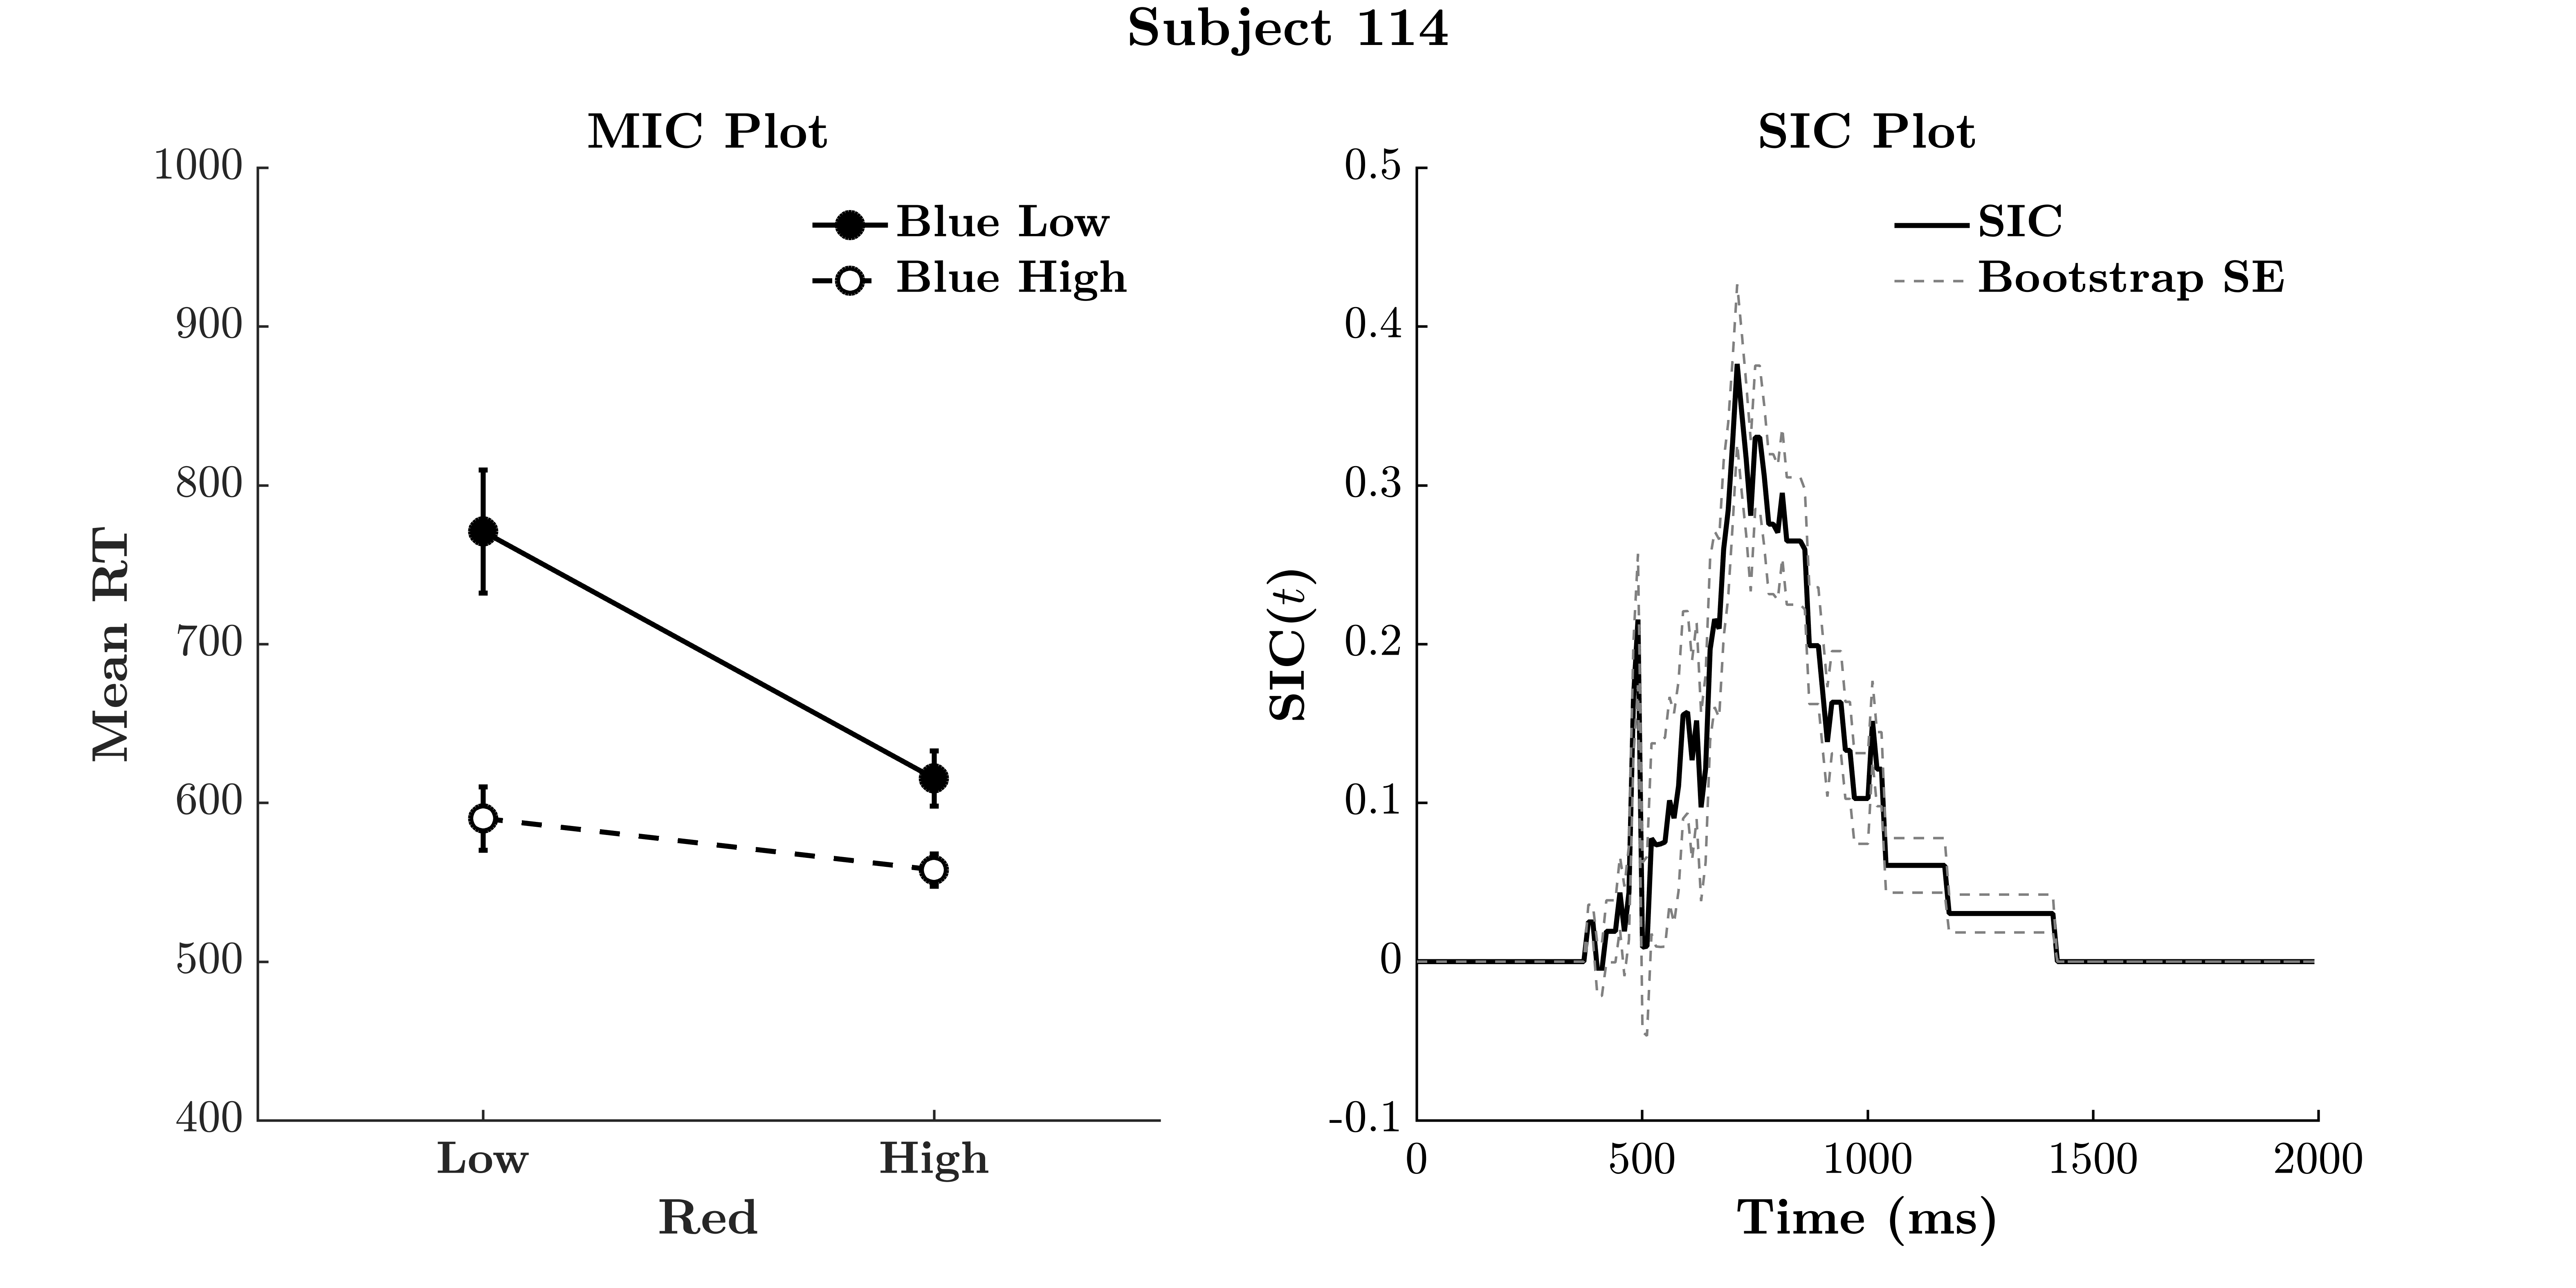
\includegraphics[width=\linewidth]{Figures/EstSystems/FIG11JPG.jpg}
\caption{Illustration of double-target mean interaction contrast (MIC; left) and survivor interaction contrast (SIC; right) plots for subject 114, displaying an over-additive MIC and a parallel minimum-time processing architecture. The MIC plot depicts mean RT for the high and low salience levels within the red and blue target color sets. Error bars represent $\pm$ one standard error of the mean. The presence of a high salience target in either color-set resulted in a fast target-present response, resulting in the illustrated interaction. By contrast, a serial or additive MIC would display no interaction. The SIC plot depicts a positive SIC function across all time points, supporting a parallel minimum-time processing architecture.}
\label{fig:EgSIC}
\end{figure}

\subsubsection{Experiment 2: Fixed Size, Divided Color-Sets}
In Experiments 2--4, processing models were diagnosed in the same way as Experiment 1. A summary of these results are reported next, and the complete results are reported in the supplementary materials S1, Table \ref{table:DT}. SIC classification supported parallel minimum-time processing in three subjects, with model probabilities $> 0.5$, and parallel minimum-time processing in one subject with a model probability $< 0.5$. One subject's data did not display selective influence at the level of the distribution, however, ordering held at the level of the mean. As such, they were subjected to MIC analysis and supported a parallel maximum-time processing architecture, confirmed by visual analysis of the MIC and a significant MIC interaction. Bayes factor analysis of the group posterior MIC provided moderately strong evidence (BF$_{10}$ = 5.11) in favor of a parallel minimum-time architecture. This result replicated in all individuals.

\subsubsection{Experiment 3: Fixed Area, Mixed Color-Sets}
After SIC categorization, three subjects displayed a parallel minimum-time processing architecture with model probabilities greater than 0.5. One subject displayed a parallel minimum-time processing architecture with an inconclusive model probability. One subject was only assessed at the level of the MIC. Bayes factor analysis of the group posterior MIC provided moderate evidence (BF$_{10}$ = 3.42) in favor of a parallel minimum-time processing architecture. This result replicated in three individuals, with two individuals displaying anecdotal evidence (BF$_{10}$ $<$ 3) in favor of parallel minimum-time processing.

\subsubsection{Experiment 4: Fixed Area, Divided Color-Sets}
After SIC classification, one subject displayed a parallel minimum-time processing architecture, and two subjects a parallel maximum-time processing architecture, with model probabilities greater than 0.5. One subject was only assessed at the level of the MIC. Bayes factor analysis of the group posterior MIC provided anecdotal evidence (BF$_{10}$ = 2.68) in favor of a parallel minimum-time processing architecture. This result replicated in two individuals. The remaining subjects provided anecdotal evidence towards a parallel maximum-time processing architecture. 

Overall, MIC and SIC results from trials in which subjects estimated two target sets ($i$.$e$., both red and blue sets had less than 20 discs each), revealed mostly parallel architecture, typically with a minimum time stopping rule (Experiments 1--3), but a maximum time stopping rule in Experiment 4. 

\section{Discussion}
When asked to estimate the quantity of two item-sets and compare them to an internal criteria, participants were able to complete the task quickly and accurately. Across the four experiments, subjects typically displayed a significant redundancy cost, and severe workload capacity limitations when estimating multiple item-sets. This capacity was so limited, as to be slower than our predictions of a theoretical serial estimation system. Workload capacity measured by the resilience function contradicted these finding, supporting an unlimited capacity, parallel estimation system. In each experiment, a limited set of subjects afforded SIC analysis of double-target responses, providing conclusive evidence that two item-sets may be estimated simultaneously through a parallel estimation-system. These results were further supported by hierarchical Bayes factor analysis, displaying moderate evidence for parallel estimation-systems.

In addressing the primary aims of this Chapter, we have determined that comparative estimation systems operate under a parallel system architecture. We determined that this parallel processing system is severely limited in workload capacity to the point that it is less-efficient than a theoretical serial estimation system. Finally, we found that these results were consistent across our conditions of item-set separability and our manipulations of item-set area. The following discussion provides a deeper breakdown on each of these elements.

\subsection{Workload Capacity}
Most subjects in Experiments 1--4 displayed a significant redundancy cost when estimating two target item-sets. This indicates that subjects had limited cognitive resources when performing estimates on multiple item-set. Capacity coefficient analysis confirmed these indications, with all subjects showing limited workload capacity, at or below the Grice lower-bound. The lower-bound is a theoretical approximation of a serial processing system. Therefore, a capacity coefficient residing at this bound indicates the system mean RT could be explained by either a serial model, or a parallel model with limited capacity. Fortunately, these are the exact mimicry conditions the SFT machinery was designed to counteract. When the lower-bound is violated --- as was the case for all subjects --- the system experiences an additional limitation to processing beyond the expectations of a serial model. This indicates the system experiences a violation of item-set $context$ $invariance$.

A parallel architecture --- as found in the current study --- could violate context invariance and yield severely limited capacity through a number of ways. Under one account, processing channels might inhibit each other, acting to slow the rate of processing in the alternate channel. In their investigation of workload, \citeauthor{eidels2011} \citeyear[Figure 3]{eidels2011} illustrated how a parallel minimum-time system with cross-channel inhibition (both pre-accumulation and post-accumulation) can predict severely limited capacity and maintain an all-positive SIC. We term this the inhibition hypothesis. 

An alternative account suggests that the rate of processing (evidence accumulation) in double-target trials is slower than in single-target trials, we term this the rate hypothesis. The rate hypothesis may occur under several conditions: (i) double-target processing-rates may slow with increases to the total stimulus set-size (the sum of red and blue items); (ii) double-target processing-rates may slow due to context effects, for example, crowding effects \cite{anobile2015mechanisms} or figure-ground segmentation effects \cite{kimchi2008figureground}. Or, (iii) double-target processing-rates may slow with the number of component item sub-sets, for example, red, blue, green and yellow item-sets. 

To test the feasibility of the rate hypothesis, we simulated a parallel model with limited capacity at the level of the accumulator using the linear ballistic accumulator (LBA) model \cite{Brown2008}. Figure \ref{fig:LimVsUnlim} illustrates \SIC and \Ct predictions when processing-rates are fixed (top panels), compared to when processing-rates are slower for double-target trials only (bottom panels). Simulated results from the slowed double-target rates, match observations from the current study. Both the inhibition hypothesis and the rate hypothesis can produce an all-positive SIC with severely limited workload capacity. To determine which hypothesis is most likely, we now consider the resilience difference function.

\begin{figure}[hbt]
\centering 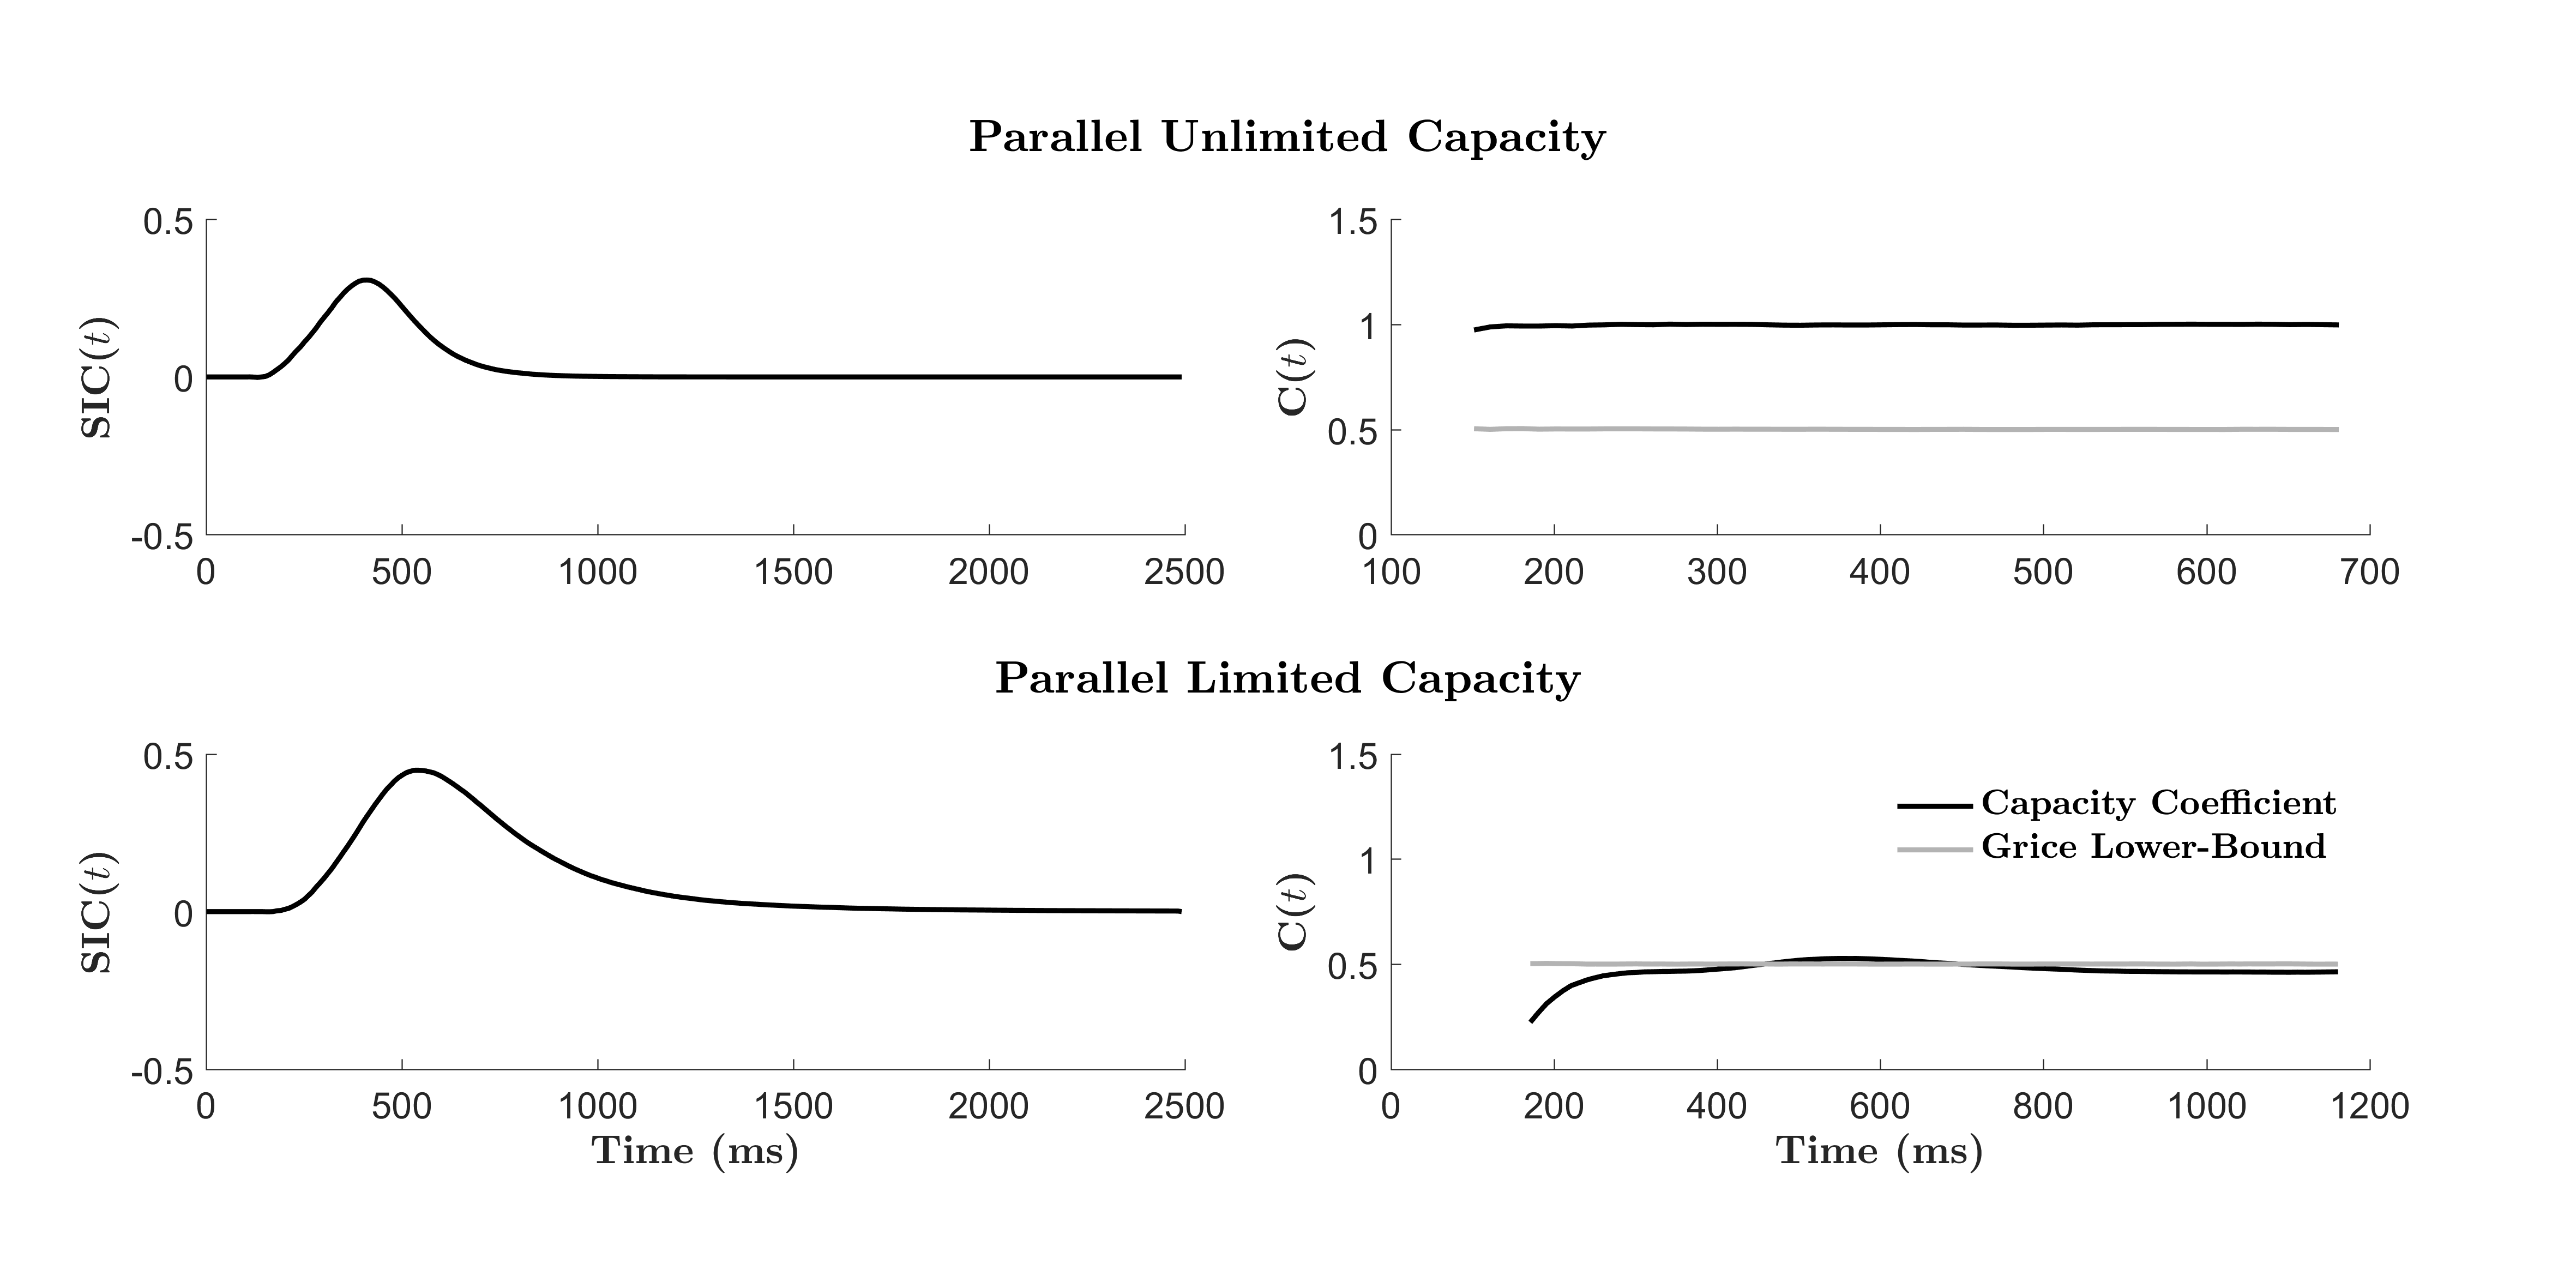
\includegraphics[width=\linewidth]{Figures/EstSystems/FIG12JPG.png}
\caption{Survivor interaction contrast SIC($t$) functions (left) and capacity coefficient C($t$) functions (right) for parallel minimum-time unlimited (top) and limited capacity (bottom) processing systems. Simulations are independent and identically distributed, and were completed with 100'000 trials per trial-type using the LBA. Threshold was set to 3, start-point 2, standard deviation 1 and non-decision time zero. Drift rates were fixed at 7 (high-salience) and 4 (low-salience), except for limited-capacity double-target trials where drift rates were reduced to 5.5 and 2.5, respectively.}
\label{fig:LimVsUnlim}
\end{figure}

\subsection{Resilience}
The resilience difference function compares the response-times for processing two-target item-sets, to the response-times for processing a target and distractor (conflict-target) item-set. Resilience difference factors out the effect of the distractor channel, providing a direct assessment of processing architecture and workload, without altering the number of processing-channels, (i.e., item-sets). Our analysis of resilience matched predictions made by an unlimited capacity, parallel processing architecture. This suggests that target processing was similar between conflict-target and double-target conditions, and that processing channels did not inhibit one another \footnote{Rdifference predictions for the inhibitory parallel model are demonstrated in \cite{Little2018mixmodel}.}. This finding directly contravenes the inhibition hypothesis. Resilience analysis also addresses a secondary question: does comparison to an internal criterion alter workload capacity. As conflict-target trials were assessed through a parallel unlimited-capacity processing system, we conclude that comparisons to an internal criterion do not alter system workload. We now consider the impact of context effects on estimation system workload capacity.

\citeA{goldfarb2013distsubitizing} observed that distractor items which could not be easily grouped, increased sub-set estimation-times. This finding aligns with our results: the presence of a redundant target-set slowed double-target response-times. Prior to this study, \citeA{HALBERDA_2006} revealed that in the presence of distractors the entire item-set was estimated $prior$ to the estimation of each item sub-set, slowing the estimation process. In line with our analyses, these findings suggest a precedence to the system workload \cite<\`a la >{navon1977forest}, with limitations occurring prior to the estimation of each item sub-set. \citeA{goldfarb2013distsubitizing} further revealed that perceptual properties, such as color and item location, were identified prior to sub-set estimation. This allows for potential context effects.

Context effects, such as the crowding effect \cite{anobile2015mechanisms} and the figure-ground segmentation effect \cite{kimchi2008figureground} disrupt single item identification and slow the rate of enumeration. Such effects are most commonly observed in dense visual scenes, for example, when more than one item-set is present. As indicated by \citeA{goldfarb2013distsubitizing}, these effects could occur prior to the enumeration of each item sub-set, slowing double-target responses relative to single-target responses. Although the separation of item-sets in Experiments 2 and 4 could allow participants to ignore the presence of an additional item-set, capacity coefficient analysis suggests this manipulation had no effect. This indicates that the item sub-sets were processed in a similar manner in both mixed and divided item-set conditions. As such, it is possible our observed limitations to workload capacity are a result of context effects occurring prior to the estimation of each item sub-set.

An alternative account of the rate hypothesis assumes that workload is limited due to the total number of items across the item sub-sets. If true, capacity should be less-limited for when the total array size is smaller than when it is larger. A comparison of estimation system workload that was sensitive enough to diagnose this difference was not possible using the current data set. Instead, we will address this account of the rate hypothesis in the following Chapter where we examine the workload capacity and processing architecture of a comparative subitizing system. 

The final condition of the rate hypothesis suggests that capacity may become more limited due to the addition of each item sub-set, for example, a red, blue and green item-set. If the capacity limitations observed in the current analysis did not violate the Grice-bound, this hypothesis could be plausible. However, the Grice-bound violation suggests that the processing of one item-set in some way inhibits the processing of the other. This inhibition requires additional cognitive constraints that go beyond the additive workload imposed by an additional item-set. For example, the context effects that may co-occur with the addition of an item-set. For this reason, any further discussion of the rate hypothesis will focused upon i) the size of the total item-set array, or ii) the impact of context effects. Having discussed our results of workload capacity, we now turn our attention to processing architecture.

\subsection{Processing Architecture}
Only a limited number of subjects met the inclusion criteria for processing architecture. As such, so we discuss results pooled across the four experiments. 

Of the fifteen subjects whose processing architecture could be conclusively assessed at the level of the SIC, all displayed a parallel processing architecture. These results align with previous findings by \citeA{HALBERDA_2006}, who used estimation acuity to theorize the parallel estimation of up to three item-sets. Results from the current study validate this theory for up to two item-sets by applying the diagnostic response-time measures of SFT.

Hierarchical Bayesian MIC analysis, conducted across a wider range of subjects, also provided moderately strong evidence in favor of parallel processing. These findings were observed at both the individual and group posterior level, and across all four experiments.

The current study is the first adaptation of the SFT framework to the study of estimation systems and came with notable limitations. In our assessment of the SIC, three subjects displayed non-determinable double-target processing architectures, and thirty-seven subjects did not meet the necessary requirement of selective influence. This suggests our manipulation of selective influence, (i.e., the numerical distance effect), was not effective for a majority of subjects. 

Through extensive testing (Chapter 2), we determined target and distractor salience levels that would ensure a high-degree of accuracy, and a significant response-time effect. As expected, we observed high accuracy in our primary task, however, our manipulation of response-time did not replicate. We suggest this effect is best explained by context effects, and small trial numbers.

As previously discussed, the presentation of multiple item-sets may have resulted in context effects that slowed item-set estimation. This effect could have compromised our manipulation of salience, leading to a lack of selective influence among the majority of tested subjects. Our manipulation of salience was particularly ineffective when item-set area was controlled, and when item-sets were separated. These manipulations may have inadvertently created a perceptual covariate of quantity, such as item-set density. This would allow subjects to identify target item-sets without engaging the ANS and our manipulation of salience. Alternately, our manipulations may have enhanced the interference produced by context effects. Both of these accounts could equally result in the poor manipulation of target salience observed within a majority of participants. 

A second limitation to our task design was the use of relatively few double-target trials \cite<compared to typical SFT studies c.f.,>{eidels2015evaluating,townsend2011}. Small trial numbers may result in unstable survivor distributions, leading to a poor manipulation of selective influence and unreliable SIC functions. As such, both small trial numbers and the presence of context effects may have contributed to our poor manipulation of salience. 

The current study faced several limitations, however, these limitations did not appear to change the fundamental processing architectures observed between Experiments. Rather, these limitations altered the number of subjects who could be diagnostically classified. As a result, it is impossible to draw strong conclusions regarding the impact of item-set area, or item-set separability, on processing architecture. 

Our findings provide conclusive evidence that double-target item-sets may be estimated through a parallel estimation system. These findings were observed by a majority of subjects whose processing architectures could be categorized. Through the novel application of SFT to an estimation task, we provide a nuanced account of the relationship between processing architecture, workload capacity and stopping-rule. Notably, we observe capacity limitations occurring before sub-set estimation, possibly caused by context effects occurring at the presentation of multiple item-sets.

These results are important, as they provide a rational for why high cognitive workload my be experienced when estimating multiple item-sets. Understanding this limitation to the human estimation system is particularly important for circumstances requiring item-set estimation under extreme or irreducible levels of workload. For example, emergency responders to a scene identifying how many people require attention, or theatre attendees choosing the fastest of two crowded exits under duress of a fire alarm. 

\subsection{Conclusion}
People often need to estimate and compare quantities, be it the number of people in line to the bank teller, party guests, or players in football teams. Little research has investigated the ability to estimate multiple quantities at the same time. Fewer still have applied machinery that can overcome parallel-serial mimicry concerns, and assess the cost to processing multiple item-sets (workload capacity). The current study is the first known attempt to apply SFT to the question of multiple-set estimation. In a series of four experiments, participants were presented with either one or two sets of 10-41 colored discs (red, blue) and had to estimate whether the number of items in each set was smaller or greater than some criterion value. SFT analyses revealed rather sever capacity limitations, meaning there was a toll in processing efficiency when subjects had to estimate the number of items in two sets relative to just one set. These results suggest that while estimation may be colloquially viewed as an effortless and possibly automatic process, the estimation of multiple item-sets is in fact a rather demanding feat. Specifically, estimating two sets was inefficient to the extent it was comparable (in terms of processing capacity) to serial processing. Understanding the fundamental cognitive mechanisms that cause this limitation is of paramount importance if we are to reduce the effective workload experienced by individuals performing multiple item-set estimates. Doing so will afford faster and more accurate estimates under difficult conditions, when we must make quick and informed approximations of quantity. This is a challenge we leave to future research.

